% block: nonhermitian-systems-heading page:111 type:section
\subsection{{非 Hermitian 线性方程组}}\label{sec:nonhermitian-linear-systems}
{回顾 CG 方法和 CR 方法 (或 MINRES 方法) 具有的以下两个良好性质:}
\begin{enumerate}
\item{残差向量满足 Ritz-Galerkin 途径 \eqref{eq:ritz-galerkin-orthogonality} 或最小残差途径 \eqref{eq:minimal-residual-problem}.}
\item{残差向量由短递推生成.}
\end{enumerate}
{如 Section\ \ref{sec:hermitian-linear-systems} 所述, 第一个性质决定近似解的最优性, 第二个性质在使每次迭代的计算开销和内存需求保持不变方面起重要作用. 回顾 Ritz--Galerkin 途径 \eqref{eq:ritz-galerkin-orthogonality} 对应于 CG 方法, 最小残差途径 \eqref{eq:minimal-residual-problem} 对应于 CR 方法和 MINRES 方法.}
% block: faber-manteuffel-limitation page:112 type:ordinary-paragraph
{\leavevmode\phantomsection\label{idx:chapter-03-section-03:faber-manteuffel-limitation}这里产生一个问题: 对于非 Hermitian 线性方程组, 是否存在同时满足这两个性质的 Krylov 子空间方法? 答案是否定的, 这已在 \BookCite{57} 中证明, 称为 Faber--Manteuffel 定理. 更具体地, 若矩阵 $A$ 具有形式}
\[A=e^{i\phi}(icI+G)\quad(c\ge0,\ 0\le\phi\le2\pi,\ B^{-1}G^{\mathrm H}B=G),\]
{则可构造同时满足这两个性质的算法. 详见 \BookCite{57} 和 Greenbaum 的著作 \BookCite{81}, Chapter 6. 另见 \BookCite{121} 及其中的参考文献.}
% block: nonhermitian-normal-equations pages:112,113 type:ordinary-paragraph
{为求解非 Hermitian 线性方程组, 可以考虑如下变换后的线性方程组:}
\begin{equation}\label{eq:nonhermitian-normal-equations}A^{\mathrm H}A\bm x=A^{\mathrm H}\bm b.\end{equation}
{若 $A$ 非奇异, 则 $A^{\mathrm H}A$ 为 Hermitian 正定矩阵. 因而可对变换后的线性方程组应用 CG 方法. 然而, $A^{\mathrm H}A$ 的条件数可能为原矩阵 $A$ 的条件数的两倍. 因此, 由 Theorem\ \ref{thm:cg-condition-number-bound}, 收敛速度可能较慢. 此外, 若条件数很大, 则由误差分析 \eqref{eq:relative-perturbation-bound} 可知, 所得近似解的精度可能很低. 注意, 误差分析 \eqref{eq:relative-perturbation-bound} 不依赖于求解线性方程组的数值算法. 这意味着, 由任何数值算法计算的近似解的精度都可能变低.}
{另一方面, 若 $A^{\mathrm H}A$ 的条件数不很大, 则有些情况下对 \eqref{eq:nonhermitian-normal-equations} 应用 CG 方法是一种可取的方法. 事实上, 若 $A$ 为酉矩阵, 则 $A^{\mathrm H}A=I$, 这表明 CG 方法只需一次迭代就给出解. 因此可以推测, 当 $A$ 接近酉矩阵时, 这一途径尤其有用. 这一途径中著名的算法为 CGNE 方法和 CGNR 方法, 将在 Section\ \ref{subsec:cg-normal-equations} 中介绍.}
{下面推导非 Hermitian 线性方程组的 Krylov 子空间方法. 将看到 BiCG 方法, BiCR 方法和 QMR 方法可分别视为 CG 方法, CR 方法和 MINRES 方法的推广, 它们基于双 Lanczos 过程 (或类似双 Lanczos 的过程); GMRES 方法可视为 MINRES 方法的推广, 且 GMRES 方法基于 Arnoldi 过程. 还将看到如何通过乘积型 Krylov 子空间方法和 IDR($s$) 方法改进 BiCG 方法.}
% block: bicg-heading page:113 type:subsection
\subsubsection{{双共轭梯度 (BiCG) 方法}}\label{subsec:bicg-method}
{与 Section\ \ref{subsec:conjugate-gradient} 中 CG 方法的推导过程类似, BiCG 方法 \BookCite{58}, \BookCite{119} 可由 Section\ \ref{subsec:bi-lanczos-process} 中的双 Lanczos 过程导出.}
{本小节给出一种简洁的推导方式, 以说明非 Hermitian 线性方程组的 BiCG 方法可从预条件 COCG 方法 (Algorithm\ \ref{alg:pcocg}) 导出. 首先考虑下列 $2N\times2N$ 复对称线性方程组:}
\begin{equation}\label{eq:bicg-augmented-system}
\begin{bmatrix}O&A\\A^{\top}&O\end{bmatrix}\begin{bmatrix}\bar{\bm x}^{*}\\\bm x\end{bmatrix}=\begin{bmatrix}\bm b\\\bar{\bm b}^{*}\end{bmatrix},\quad\text{or }\widetilde A\widetilde{\bm x}=\widetilde{\bm b}.
\end{equation}
{由方程组 \eqref{eq:bicg-augmented-system} 可看出, 它在数学上等价于}
\[A\bm x=\bm b\quad\text{and}\quad A^{\top}\bar{\bm x}^{*}=\bar{\bm b}^{*}\quad(\Leftrightarrow A^{\mathrm H}\bm x^{*}=\bm b^{*}).\]
{若采用下列预条件子, 将 COCG 算法}
\begin{equation}\label{eq:bicg-swap-preconditioner}\widetilde M=\begin{bmatrix}O&I\\I&O\end{bmatrix},\quad I:\text{ identity matrix},\end{equation}
{应用于 \eqref{eq:bicg-augmented-system}, 则所得算法在第 $n$ 次迭代时可写为}
% block: bicg-augmented-cocg-recurrences page:114 type:ordinary-paragraph
\[\begin{aligned}
\widetilde{\bm p}_n^{\mathrm{COCG}}&=\widetilde M^{-1}\widetilde{\bm r}_n^{\mathrm{COCG}}+\beta_{n-1}\widetilde{\bm p}_{n-1}^{\mathrm{COCG}},\\
\alpha_n&=\frac{(\overline{\widetilde M^{-1}\widetilde{\bm r}_n^{\mathrm{COCG}}},\widetilde{\bm r}_n^{\mathrm{COCG}})}{(\overline{\widetilde{\bm p}_n^{\mathrm{COCG}}},\widetilde A\widetilde{\bm p}_n^{\mathrm{COCG}})},\\
\widetilde{\bm x}_{n+1}^{\mathrm{COCG}}&=\widetilde{\bm x}_n^{\mathrm{COCG}}+\alpha_n\widetilde{\bm p}_n^{\mathrm{COCG}},\\
\widetilde{\bm r}_{n+1}^{\mathrm{COCG}}&=\widetilde{\bm r}_n^{\mathrm{COCG}}-\alpha_n\widetilde A\widetilde{\bm p}_n^{\mathrm{COCG}},\\
\beta_n&=\frac{(\overline{\widetilde M^{-1}\widetilde{\bm r}_{n+1}^{\mathrm{COCG}}},\widetilde{\bm r}_{n+1}^{\mathrm{COCG}})}{(\overline{\widetilde M^{-1}\widetilde{\bm r}_n^{\mathrm{COCG}}},\widetilde{\bm r}_n^{\mathrm{COCG}})}.
\end{aligned}\]
{将 \eqref{eq:bicg-swap-preconditioner} 中的 $\widetilde M^{-1}(=\widetilde M)$ 及向量}
\[\widetilde{\bm x}_n^{\mathrm{COCG}}:=\begin{bmatrix}\bm x_n\\\bar{\bm x}_n^{*}\end{bmatrix},\quad\widetilde{\bm r}_n^{\mathrm{COCG}}:=\begin{bmatrix}\bm r_n\\\bar{\bm r}_n^{*}\end{bmatrix},\quad\widetilde{\bm p}_n^{\mathrm{COCG}}:=\begin{bmatrix}\bar{\bm p}_n^{*}\\\bm p_n\end{bmatrix}\]
{代入前述递推式, 并使用下列结果:}
\[\begin{aligned}
(\overline{\widetilde M^{-1}\widetilde{\bm r}_n^{\mathrm{COCG}}},\widetilde{\bm r}_n^{\mathrm{COCG}})&=\begin{bmatrix}\bar{\bm r}_n^{*\top}&\bm r_n^{\top}\end{bmatrix}\begin{bmatrix}\bm r_n\\\bar{\bm r}_n^{*}\end{bmatrix}\\
&=\bar{\bm r}_n^{*\top}\bm r_n+\bm r_n^{\top}\bar{\bm r}_n^{*}\\
&=\bm r_n^{*\mathrm H}\bm r_n+(\bm r_n^{\top}\bar{\bm r}_n^{*})^{\top}\\
&=(\bm r_n^{*},\bm r_n)+\bm r_n^{*\mathrm H}\bm r_n\\
&=2(\bm r_n^{*},\bm r_n)\\
(\overline{\widetilde{\bm p}_n^{\mathrm{COCG}}},\widetilde A\widetilde{\bm p}_n^{\mathrm{COCG}}),&=\begin{bmatrix}((\bar{\bm p}_n^{*})^{\top}\bm p_n)^{\top}\end{bmatrix}\begin{bmatrix}A\bm p_n\\A^{\top}\bar{\bm p}_n^{*}\end{bmatrix}\\
&=(\bm p_n^{*})^{\mathrm H}A\bm p_n+\bm p_n^{\top}A^{\top}\bar{\bm p}_n^{*},\\
&=(\bm p_n^{*})^{\mathrm H}A\bm p_n+(\bm p_n^{\top}A^{\top}\bar{\bm p}_n^{*})^{\top},\\
&=2(\bm p_n^{*},A\bm p_n),
\end{aligned}\]
{就容易得到 Algorithm\ \ref{alg:bicg} 所述的求解非 Hermitian 线性方程组的 BiCG 算法. 若矩阵 $A$ 为实非对称矩阵, 则上述推导过程对应于 van der Vorst 的著作 \BookCite{196}, Chapter 7 中的推导, 其中实非对称线性方程组的 BiCG 方法由 CG 方法导出.}
{由 Algorithm\ \ref{alg:bicg} 可见, 若系数矩阵 $A$ 为 Hermitian 矩阵, 则选择 $\bm r_0^{*}=\bm r_0$ 就退化为 CG 方法.}
% block: bicg-biorthogonality-proposition page:114 type:proposition
{与 Proposition\ \ref{prop:cg-orthogonality} 所示的 CG 迭代类似, BiCG 迭代具有下列关系:}
\par\Needspace{3\baselineskip}
\begin{Proposition}\label{prop:bicg-biorthogonality}
{设 $\bm p_n,\bm r_n$ 为 BiCG 方法中的向量. 则,}
\begin{enumerate}\item $(\bm r_i^{*},\bm r_j)=0\quad\text{for }i\ne j$,\item $(\bm p_i^{*},A\bm p_j)=0\quad\text{for }i\ne j$.\end{enumerate}
\end{Proposition}
% block: bicg-algorithm page:115 type:ordinary-paragraph
\begin{algorithm}[H]\caption{{BiCG 方法}}\label{alg:bicg}\begin{algorithmic}[1]
\Statex\textbf{Input:} $\bm x_0\in\mathbb C^N,\ \beta_{-1}=0,\ \bm p_{-1}=\bm p_{-1}^{*}=\bm0,\ \bm r_0=\bm b-A\bm x_0$
\Statex\textbf{Input:} {选择 $\bm r_0^{*}\in\mathbb C^N$, 例如 $\bm r_0^{*}=\bm r_0$}
\Statex\textbf{Output:} $\bm x_n$
\For{$n=0,1,2,\ldots$, {直至收敛}}
\State $\bm p_n=\bm r_n+\beta_{n-1}\bm p_{n-1},\quad\bm p_n^{*}=\bm r_n^{*}+\bar\beta_{n-1}\bm p_{n-1}^{*}$
\State $\alpha_n=\frac{(\bm r_n^{*},\bm r_n)}{(\bm p_n^{*},A\bm p_n)}$
\State $\bm x_{n+1}=\bm x_n+\alpha_n\bm p_n$
\State $\bm r_{n+1}=\bm r_n-\alpha_nA\bm p_n,\quad\bm r_{n+1}^{*}=\bm r_n^{*}-\bar\alpha_nA^{\mathrm H}\bm p_n^{*}$
\State $\beta_n=\frac{(\bm r_{n+1}^{*},\bm r_{n+1})}{(\bm r_n^{*},\bm r_n)}$
\EndFor\end{algorithmic}\end{algorithm}
% block: bicg-krylov-corollary page:115 type:corollary
{由 Proposition\ \ref{prop:bicg-biorthogonality}, 下列性质成立:}
\par\Needspace{3\baselineskip}
\begin{Corollary}\label{cor:bicg-krylov-orthogonality}
{设 $\bm p_n,\bm r_n$ 为 BiCG 方法中的向量. 则,}
\begin{enumerate}\item $\bm r_n\perp\mathcal K_n(A^{\mathrm H},\bm r_0^{*})$,\item $A\bm p_n\perp\mathcal K_n(A^{\mathrm H},\bm r_0^{*})$.\end{enumerate}
\end{Corollary}
% block: bicg-alternative-alpha page:115 type:ordinary-paragraph
{下面给出 BiCG 方法中 $\alpha_n$ 和 $\beta_n$ 的其他计算公式, 它们将用于推导 Section\ \ref{subsec:product-type-krylov} 中的乘积型 Krylov 子空间方法.}
{由于 $\bm r_n^{*}\in\mathcal K_{n+1}(A^{\mathrm H},\bm r_0^{*})$, 向量 $\bm r_n^{*}$ 可写为}
\[\begin{aligned}\bm r_n^{*}&=c_n(A^{\mathrm H})^n\bm r_0^{*}+\underbrace{c_{n-1}(A^{\mathrm H})^{n-1}\bm r_0^{*}+\cdots+c_0\bm r_0^{*}}_{\bm z}\\&=c_n(A^{\mathrm H})^n\bm r_0^{*}+\bm z,\quad\bm z\in\mathcal K_n(A^{\mathrm H},\bm r_0^{*}).\end{aligned}\]
{由上式及 Corollary\ \ref{cor:bicg-krylov-orthogonality} 得}
\[\begin{aligned}(\bm r_n^{*},\bm r_n)&=(c_n(A^{\mathrm H})^n\bm r_0^{*}+\bm z,\bm r_n)=\bar c_n((A^{\mathrm H})^n\bm r_0^{*},\bm r_n)+(\bm z,\bm r_n)\\&=\bar c_n((A^{\mathrm H})^n\bm r_0^{*},\bm r_n)\\
(\bm r_n^{*},A\bm p_n)&=(c_n(A^{\mathrm H})^n\bm r_0^{*}+\bm z,A\bm p_n)=\bar c_n((A^{\mathrm H})^n\bm r_0^{*},A\bm p_n)+(\bm z,A\bm p_n)\\&=\bar c_n((A^{\mathrm H})^n\bm r_0^{*},A\bm p_n).
\end{aligned}\]
{因此, BiCG 方法 (Algorithm\ \ref{alg:bicg}) 的 $\alpha_n$ 可改写为}
\begin{equation}\label{eq:bicg-alpha-shadow-power}\alpha_n=\frac{(\bm r_n^{*},\bm r_n)}{(\bm p_n^{*},A\bm p_n)}=\frac{((A^{\mathrm H})^n\bm r_0^{*},\bm r_n)}{((A^{\mathrm H})^n\bm r_0^{*},A\bm p_n)}.\end{equation}
% block: bicg-alternative-beta pages:115,116 type:ordinary-paragraph
{类似地, 给出 $\beta_n$ 的其他计算公式. 由 Corollary\ \ref{cor:bicg-krylov-orthogonality}, 两个向量 $(A^{\mathrm H})^n\bm r_0^{*}\in\mathcal K_{n+1}(A^{\mathrm H},\bm r_0^{*})$ 和 $A\bm p_{n+1}$ 正交, 因此}
\[\begin{aligned}0&=((A^{\mathrm H})^n\bm r_0^{*},A\bm p_{n+1})\\&=((A^{\mathrm H})^n\bm r_0^{*},A\bm r_{n+1}+\beta_nA\bm p_n)\\&=((A^{\mathrm H})^n\bm r_0^{*},A\bm r_{n+1})+\beta_n((A^{\mathrm H})^n\bm r_0^{*},A\bm p_n)\\&=((A^{\mathrm H})^{n+1}\bm r_0^{*},\bm r_{n+1})+\beta_n((A^{\mathrm H})^n\bm r_0^{*},A\bm p_n),\end{aligned}\]
{立即得到}
\[\beta_n=-\frac{((A^{\mathrm H})^{n+1}\bm r_0^{*},\bm r_{n+1})}{((A^{\mathrm H})^n\bm r_0^{*},A\bm p_n)}.\]
{结合 \eqref{eq:bicg-alpha-shadow-power} 与上述结果, 得}
\begin{equation}\label{eq:bicg-beta-shadow-power}\beta_n=-\alpha_n\frac{((A^{\mathrm H})^{n+1}\bm r_0^{*},\bm r_{n+1})}{((A^{\mathrm H})^n\bm r_0^{*},\bm r_n)}.\end{equation}
% block: composite-step-bicg-heading page:116 type:subsection
\subsubsection{{复合步双共轭梯度 (CSBiCG) 方法}}\label{subsec:composite-step-bicg}
{由 BiCG 方法的算法 (Algorithm\ \ref{alg:bicg}), 有两类可能的 (近) 中断:}
\begin{enumerate}
\item $\rho_n:=(\bm r_n^{*},\bm r_n)=0$ {而 $\bm r_n\ne\bm0$ (Lanczos 中断),}
\item $\sigma_n:=(\bm p_n^{*},A\bm p_n)=0$ ({主元中断}).
\end{enumerate}
{Lanczos 中断可通过 \BookCite{145}, \BookCite{189} 中的前瞻 Lanczos 过程避免. Bank 和 Chan 关注主元中断, 在假设不发生 Lanczos 中断的条件下, 提出复合步双共轭梯度 (CSBiCG) 方法来消除主元中断 \BookCite{16}, \BookCite{17}. 下面根据 \BookCite{17} 对该算法作简要说明.}
% block: composite-step-auxiliary-vectors pages:116,117 type:ordinary-paragraph
{若 $\sigma_n=0$, 就无法得到 $\bm r_{n+1}=\bm r_n-(\rho_n/\sigma_n)A\bm p_n$ 和 $\bm r_{n+1}^{*}=\bm r_n^{*}-\overline{(\rho_n/\sigma_n)}A^{\mathrm H}\bm p_n^{*}$. 考虑辅助向量:}
\[\begin{aligned}\bm z_{n+1}&=\sigma_n\bm r_n-\rho_nA\bm p_n,\\\bm z_{n+1}^{*}&=\bar\sigma_n\bm r_n-\bar\rho_nA^{\mathrm H}\bm p_n^{*}.\end{aligned}\]
{于是即使 $\sigma_n=0$, $\bm z_{n+1}$ 和 $\bm z_{n+1}^{*}$ 也存在, 且 $\bm z_{n+1}$ 和 $\bm z_{n+1}^{*}$ 分别属于 $\mathcal K_{n+2}(A,\bm r_0)$ 和 $\mathcal K_{n+2}(A^{\mathrm H},\bm r_0^{*})$. 随后复合步技术按下式考虑 $\bm r_{n+2}$ 和 $\bm r_{n+2}^{*}$:}
\[\begin{aligned}\bm r_{n+2}&=\bm r_n-c_1A\bm p_n-c_2A\bm z_{n+1},\\\bm r_{n+2}^{*}&=\bm r_n^{*}-c_1^{*}A^{\mathrm H}\bm p_n^{*}-c_2^{*}A^{\mathrm H}\bm z_{n+1}^{*},\end{aligned}\]
{其中 $c_1,c_2,c_1^{*},c_2^{*}$ 确定为使得}
\[\bm r_{n+2}\perp\operatorname{span}\{\bm p_n^{*},\bm z_{n+1}^{*}\},\qquad\bm r_{n+2}^{*}\perp\operatorname{span}\{\bm p_n,\bm z_{n+1}\},\]
{即 $(\bm r_{n+2},\bm p_n^{*})=(\bm r_{n+2},\bm z_{n+1}^{*})=(\bm r_{n+2}^{*},\bm p_n)=(\bm r_{n+2}^{*},\bm z_{n+1})=0$. 类似地, 令}
\[\begin{aligned}\bm p_{n+2}&=\bm r_{n+2}+d_1\bm p_n+d_2\bm z_{n+1},\\\bm p_{n+2}^{*}&=\bm r_{n+2}^{*}+d_1^{*}\bm p_n^{*}+d_2^{*}\bm z_{n+1}^{*},\end{aligned}\]
{并确定 $d_1,d_2,d_1^{*},d_2^{*}$ 使得}
\[A\bm p_{n+2}\perp\operatorname{span}\{\bm p_n^{*},\bm z_{n+1}^{*}\},\qquad A^{\mathrm H}\bm p_{n+2}^{*}\perp\operatorname{span}\{\bm p_n,\bm z_{n+1}\}.\]
{于是 \BookCite{17}, Theorem 4.4 说明, 当 $i\ne j$ 时有 $(\bm r_i^{*},\bm r_j)=(\bm p_i^{*},A\bm p_j)=0$, 这意味着复合步残差向量 $\bm r_{n+2}$ 和 $A\bm p_{n+2}$ 满足}
\[\bm r_{n+2}\perp\mathcal K_{n+2}(A^{\mathrm H},\bm r_0^{*}),\quad A\bm p_{n+2}\perp\mathcal K_{n+2}(A^{\mathrm H},\bm r_0^{*}).\]
{这些与 BiCG 方法具有的性质相同, 见 Corollary\ \ref{cor:bicg-krylov-orthogonality}. 所得算法见 Algorithm\ \ref{alg:composite-step-bicg}.}
% block: composite-step-choice page:117 type:ordinary-paragraph
{由 Algorithm\ \ref{alg:composite-step-bicg}, 矩阵向量乘法的次数与 BiCG 方法相同. 复合步技术也用于其他 Krylov 子空间方法 \BookCite{35}, \BookCite{113}.}
{在 Algorithm\ \ref{alg:composite-step-bicg} 的每一步, 需要选择 $1\times1$ 步 (BiCG 步) 或 $2\times2$ 步 (复合步). 文献 \BookCite{17} 提出如下选择:}
\begin{algorithmic}[1]
\If{$\|\bm z_{n+1}\|\le\|\bm r_n\||\sigma_n|$}
\State $1\times1$ {步}
\Else
\State $\nu_{n+2}=\|\delta_n\bm r_n-\rho_n^3\zeta_{n+1}\bm q_n-\theta_{n+1}\rho_n^2\bm y_{n+1}\|$
\If{$\nu_{n+2}|\sigma_n|<\|\bm z_{n+1}\||\delta_n|$}
\State $2\times2$ {步}
\Else\State $1\times1$ {步}\EndIf\EndIf
\end{algorithmic}
{这一选择不仅避免 (近) 主元中断, 也使残差范数的收敛历程得到一定程度的平滑.}
% block: composite-step-bicg-algorithm page:118 type:ordinary-paragraph
\begin{algorithm}[H]\caption{{复合步 BiCG 方法}}\label{alg:composite-step-bicg}\begin{algorithmic}[1]
\Statex\textbf{Input:} $\bm x_0\in\mathbb C^N,\ \bm r_0=\bm b-A\bm x_0$
\Statex\textbf{Input:} {选择 $\bm r_0^{*}\in\mathbb C^N$, 例如 $\bm r_0^{*}=\bm r_0$}
\Statex\textbf{Output:} $\bm x_n$
\State $\bm p_0=\bm r_0,\quad\bm p_0^{*}=\bm r_0^{*}$
\State $\bm q_0=A\bm p_0,\quad\bm q_0^{*}=A^{\mathrm H}\bm p_0^{*}$
\State $\rho_0=(\bm r_0^{*},\bm r_0)$
\State $n=0$
\While{{直至收敛}}
\State $\sigma_n=(\bm p_n^{*},\bm q_n)$
\State $\bm z_{n+1}=\sigma_n\bm r_n-\rho_n\bm q_n,\quad\bm z_{n+1}^{*}=\bar\sigma_n\bm r_n^{*}-\bar\rho_n\bm q_n^{*}$
\State $\bm y_{n+1}=A\bm z_{n+1},\quad\bm y_{n+1}^{*}=A^{\mathrm H}\bm z_{n+1}^{*}$
\State $\theta_{n+1}=(\bm z_{n+1}^{*},\bm z_{n+1})$
\State $\zeta_{n+1}=(\bm z_{n+1}^{*},\bm y_{n+1})$
\If{$1\times1$ {步}}
\State $\alpha=\rho_n/\sigma_n$
\State $\rho_{n+1}=\theta_{n+1}/\sigma_n^2$
\State $\beta_{n+1}=\rho_{n+1}/\rho_n$
\State $\bm x_{n+1}=\bm x_n+\alpha_n\bm p_n$
\State $\bm r_{n+1}=\bm r_n-\alpha_n\bm q_n,\quad\bm r_{n+1}^{*}=\bm r_n^{*}-\bar\alpha_n\bm q_n^{*}$
\State $\bm p_{n+1}=\bm z_{n+1}/\sigma_n+\beta_{n+1}\bm p_n,\quad\bm p_{n+1}^{*}=\bm z_{n+1}^{*}/\bar\sigma_n+\bar\beta_{n+1}\bm p_n^{*}$
\State $\bm q_{n+1}=\bm y_{n+1}/\sigma_n+\beta_{n+1}\bm q_n,\quad\bm q_{n+1}^{*}=\bm y_{n+1}^{*}/\bar\sigma_n+\bar\beta_{n+1}\bm q_n^{*}$
\State $n=n+1$
\EndIf
\If{$2\times2$ {步}}
\State $\delta_n=\sigma_n\zeta_{n+1}\rho_n^2-\theta_{n+1}^2$
\State $\alpha_n=\zeta_{n+1}\rho_n^3/\delta_n,\quad\alpha_{n+1}=\theta_{n+1}\rho_n^2/\delta_n$
\State $\bm x_{n+2}=\bm x_n+\alpha_n\bm p_n+\alpha_{n+1}\bm z_{n+1}$
\State $\bm r_{n+2}=\bm r_n-\alpha_n\bm q_n-\alpha_{n+1}\bm y_{n+1},\quad\bm r_{n+2}^{*}=\bm r_n^{*}-\bar\alpha_n\bm q_n^{*}-\bar\alpha_{n+1}\bm y_{n+1}$
\State $\rho_{n+2}=(\bm r_{n+2}^{*},\bm r_{n+2})$
\State $\beta_{n+1}=\rho_{n+2}/\rho_n,\quad\beta_{n+2}=\rho_{n+2}\sigma_n/\theta_{n+1}$
\State $\bm p_{n+2}=\bm r_{n+2}+\beta_{n+1}\bm p_n+\beta_{n+2}\bm z_{n+1},\quad\bm p_{n+2}^{*}=\bm r_{n+2}^{*}+\bar\beta_{n+1}\bm p_n^{*}+\bar\beta_{n+2}\bm z_{n+1}^{*}$
\State $\bm q_{n+2}=A\bm p_{n+2},\quad\bm q_{n+2}^{*}=A^{\mathrm H}\bm p_{n+2}^{*}$
\State $n=n+2$
\EndIf\EndWhile\end{algorithmic}\end{algorithm}
% block: composite-bicg-best-approximation pages:118,119 type:theorem
{下述定理给出 (复合步) BiCG 方法的最佳逼近结果:}
\par\Needspace{14\baselineskip}
\begin{Theorem}[\BookCite{16}]\label{thm:composite-bicg-best-approximation}
{考虑对实非对称线性方程组应用 (复合步) BiCG 方法, 初始猜测为 $\bm x_0=\bm0$, 且 $\bm r_0^{*}=\bm r_0$. 假设对所有 $\bm v,\bm w\in\mathbb R^N$, 有}
\[|\bm w^{\top}A\bm v|\le\Gamma\|\bm v\|\|\bm w\|,\]
{其中 $\Gamma$ 为与 $\bm v$ 和 $\bm w$ 无关的常数. 进一步假设, 对于 (复合步) BiCG 方法中计算近似解 $\bm x_n$ 的那些步骤, 有}
\[\inf_{\substack{\bm v\in\mathcal K_n(A,\bm r_0)\\\|\bm v\|=1}}\ \sup_{\substack{\bm w\in\mathcal K_n(A^{\top},\bm r_0^{*})\\\|\bm w\|\le1}}\bm w^{\top}A\bm v\ge\delta_n\ge\delta>0.\]
{则}
\[\|\bm x-\bm x_n\|\le(1+\Gamma/\delta)\inf_{\bm v\in\mathcal K_n(A,\bm r_0)}\|\bm x-\bm v\|.\]
\end{Theorem}
{Theorem\ \ref{thm:composite-bicg-best-approximation} 是 \BookCite{16} 中 Theorem 4.1 的简化结果. 由 Theorem\ \ref{thm:composite-bicg-best-approximation} 可见, 当 $\Gamma/\delta$ 接近 0 时, (复合步) BiCG 方法产生在误差范数下接近最佳近似解的近似解.}
% block: bicr-heading page:119 type:subsection
\subsubsection{{双共轭残差 (BiCR) 方法}}\label{subsec:bicr-method}
{BiCR 方法 \BookCite{169} 是 CR 方法向非 Hermitian 线性方程组的推广.}\footnote{{Chronopulous 和 Ma 于 1989 年的未发表论文 \BookCite{38} 中提到了该方法, Chronopulous 博士于 2020 年 4 月 6 日通过电子邮件将这一事实告知作者.}}
{本小节说明 BiCR 方法可由 Algorithm\ \ref{alg:pcocr} 中的预条件 COCR 方法导出. 采用预条件子 \eqref{eq:bicg-swap-preconditioner}, 对 \eqref{eq:bicg-augmented-system} 应用 COCR 算法, 所得算法在第 $n$ 次迭代时可写为}
\[\begin{aligned}
\widetilde{\bm p}_n^{\mathrm{COCR}}&=\widetilde M^{-1}\widetilde{\bm r}_n^{\mathrm{COCR}}+\beta_{n-1}\widetilde{\bm p}_{n-1}^{\mathrm{COCR}},\\
\alpha_n&=\frac{(\overline{\widetilde M^{-1}\widetilde{\bm r}_n^{\mathrm{COCR}}},\widetilde A\widetilde M^{-1}\widetilde{\bm r}_n^{\mathrm{COCR}})}{(\overline{\widetilde A\widetilde{\bm p}_n^{\mathrm{COCR}}},\widetilde M^{-1}\widetilde A\widetilde{\bm p}_n^{\mathrm{COCR}})},\\
\widetilde{\bm x}_{n+1}^{\mathrm{COCR}}&=\widetilde{\bm x}_n^{\mathrm{COCR}}+\alpha_n\widetilde{\bm p}_n^{\mathrm{COCR}},\\
\widetilde{\bm r}_{n+1}^{\mathrm{COCR}}&=\widetilde{\bm r}_n^{\mathrm{COCR}}-\alpha_n\widetilde A\widetilde{\bm p}_n^{\mathrm{COCR}},\\
\beta_n&=\frac{(\overline{\widetilde M^{-1}\widetilde{\bm r}_{n+1}^{\mathrm{COCR}}},\widetilde A\widetilde M^{-1}\widetilde{\bm r}_{n+1}^{\mathrm{COCR}})}{(\overline{\widetilde M^{-1}\widetilde{\bm r}_n^{\mathrm{COCR}}},\widetilde A\widetilde M^{-1}\widetilde{\bm r}_n^{\mathrm{COCR}})}.
\end{aligned}\]
{将 \eqref{eq:bicg-swap-preconditioner} 中的 $\widetilde M^{-1}(=\widetilde M)$ 以及向量}
\[\widetilde{\bm x}_n^{\mathrm{COCR}}:=\begin{bmatrix}\bm x_n\\\bar{\bm x}_n^{*}\end{bmatrix},\quad\widetilde{\bm r}_n^{\mathrm{COCR}}:=\begin{bmatrix}\bm r_n\\\bar{\bm r}_n^{*}\end{bmatrix},\quad\widetilde{\bm p}_n^{\mathrm{COCR}}:=\begin{bmatrix}\bar{\bm p}_n^{*}\\\bm p_n\end{bmatrix}\]
{代入前述递推式, 并使用下列结果:}
% block: bicr-bilinear-reductions page:120 type:ordinary-paragraph
\[\begin{aligned}
(\overline{\widetilde M^{-1}\widetilde{\bm r}_n^{\mathrm{COCR}}},\widetilde A\widetilde M^{-1}\widetilde{\bm r}_n^{\mathrm{COCR}})&=\begin{bmatrix}\bar{\bm r}_n^{*\top}&\bm r_n^{\top}\end{bmatrix}\begin{bmatrix}A\bm r_n\\A^{\top}\bar{\bm r}_n^{*}\end{bmatrix}\\
&=\bar{\bm r}_n^{*\top}A\bm r_n+\bm r_n^{\top}A^{\top}\bar{\bm r}_n^{*}\\
&=\bm r_n^{*\mathrm H}A\bm r_n+(\bm r_n^{\top}A^{\top}\bar{\bm r}_n^{*})^{\top}\\
&=(\bm r_n^{*},A\bm r_n)+\bm r_n^{*\mathrm H}A\bm r_n\\
&=2(\bm r_n^{*},A\bm r_n)
\end{aligned}\]
{以及}
\[\begin{aligned}
(\overline{\widetilde A\widetilde{\bm p}_n^{\mathrm{COCR}}},\widetilde M^{-1}\widetilde A\widetilde{\bm p}_n^{\mathrm{COCR}})&=\begin{bmatrix}(A\bm p_n)^{\top}&(A^{\top}\bar{\bm p}_n^{*})^{\top}\end{bmatrix}\begin{bmatrix}A^{\top}\bar{\bm p}_n^{*}\\A\bm p_n\end{bmatrix}\\
&=(A\bm p_n)^{\top}A^{\top}\bar{\bm p}_n^{*}+(A^{\top}\bar{\bm p}_n^{*})^{\top}A\bm p_n\\
&=(\bm p_n^{\top}A^{\top}A^{\top}\bar{\bm p}_n^{*})^{\top}+(A^{\mathrm H}\bm p_n^{*})^{\mathrm H}A\bm p_n\\
&=(A^{\mathrm H}\bm p_n^{*})^{\mathrm H}A\bm p_n+(A^{\mathrm H}\bm p_n^{*},A\bm p_n)\\
&=2(A^{\mathrm H}\bm p_n^{*},A\bm p_n),
\end{aligned}\]
{就容易得到求解非 Hermitian 线性方程组的 BiCR 算法.}
% block: bicr-algorithm page:120 type:ordinary-paragraph
\begin{algorithm}[H]\caption{{BiCR 方法}}\label{alg:bicr}\begin{algorithmic}[1]
\Statex\textbf{Input:} $\bm x_0\in\mathbb C^N,\ \beta_{-1}=0,\ \bm p_{-1}=\bm p_{-1}^{*}=\bm0,\ \bm r_0=\bm b-A\bm x_0$
\Statex\textbf{Input:} {选择 $\bm r_0^{*}\in\mathbb C^N$, 例如 $\bm r_0^{*}=\bm r_0$}
\Statex\textbf{Output:} $\bm x_n$
\For{$n=0,1,2,\ldots$, {直至收敛}}
\State $\bm p_n=\bm r_n+\beta_{n-1}\bm p_{n-1},\quad\bm p_n^{*}=\bm r_n^{*}+\bar\beta_{n-1}\bm p_{n-1}^{*}$
\State $A\bm p_n=A\bm r_n+\beta_{n-1}A\bm p_{n-1}$
\State $\alpha_n=\frac{(\bm r_n^{*},A\bm r_n)}{(A^{\mathrm H}\bm p_n^{*},A\bm p_n)}$
\State $\bm x_{n+1}=\bm x_n+\alpha_n\bm p_n$
\State $\bm r_{n+1}=\bm r_n-\alpha_nA\bm p_n,\quad\bm r_{n+1}^{*}=\bm r_n^{*}-\bar\alpha_nA^{\mathrm H}\bm p_n^{*}$
\State $\beta_n=\frac{(\bm r_{n+1}^{*},A\bm r_{n+1})}{(\bm r_n^{*},A\bm r_n)}$
\EndFor\end{algorithmic}\end{algorithm}
% block: bicr-biorthogonality-proposition page:120 type:proposition
{与 Proposition\ \ref{prop:bicg-biorthogonality} 类似, BiCR 迭代具有以下性质:}
\par\Needspace{3\baselineskip}
\begin{Proposition}\label{prop:bicr-biorthogonality}
{设 $\bm p_n,\bm r_n$ 为 BiCR 方法中的向量. 则,}
\begin{enumerate}\item $(\bm r_i^{*},A\bm r_j)=0\quad\text{for }i\ne j$,\item $(A^{\mathrm H}\bm p_i^{*},A\bm p_j)=0\quad\text{for }i\ne j$.\end{enumerate}
\end{Proposition}
{若系数矩阵 $A$ 为 Hermitian 矩阵或实对称矩阵, 则选择 $\bm r_0^{*}=\bm r_0$ 就退化为 CR 方法, 后者产生残差 2-范数意义下的最优近似解. 因此, 若 $A$ 接近 Hermitian 矩阵或实对称矩阵, 可以预期 BiCR 方法具有平滑的收敛行为, 并产生接近最小残差的解.}
% block: bicr-convergence-comparison page:121 type:ordinary-paragraph
{为说明这一点, 考虑非对称线性方程组 \eqref{eq:three-dimensional-difference-system}, 参数为 $N=20$, $a_1=a_2=a_3=1$, 两组不同的数值 $b_1=b_2=b_3=0.1$ (接近对称的矩阵) 和 $b_1=b_2=b_3=10$ (远离对称的矩阵), 以及 $c=700$. 横轴为矩阵向量乘法的次数. BiCG 方法和 BiCR 方法所用的停止准则为 $\|\bm r_n\|/\|\bm b\|\le10^{-10}$.}
{当 $b_1=b_2=b_3=0.1$ (接近对称的矩阵) 时的结果见 Figure\ \ref{fig:bicg-bicr-near-symmetric}. 从 Figure\ \ref{fig:bicg-bicr-near-symmetric} 可见, BiCR 方法表现出的收敛行为比 BiCG 方法平滑得多.}
{当 $b_1=b_2=b_3=0.1$ (远离对称的矩阵) 时的结果见 Figure\ \ref{fig:bicg-bicr-far-symmetric}. 从 Figure\ \ref{fig:bicg-bicr-far-symmetric} 可见, BiCG 方法和 BiCR 方法具有相似的收敛行为, BiCR 方法未表现出平滑的收敛行为.}
% block: bicr-near-symmetric-figure page:121 type:figure
\begin{figure}[H]\centering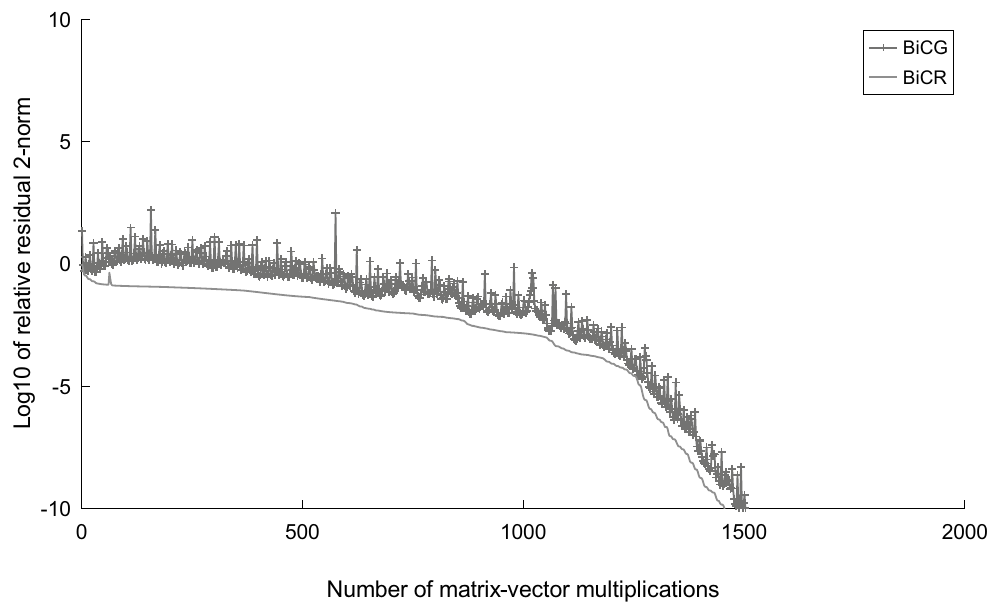
\includegraphics[width=.87\linewidth]{figures/bicg-bicr-near-symmetric.png}
\caption{{当 $b_1=b_2=b_3=0.1$ 时 BiCG 和 BiCR 的收敛历程}}\label{fig:bicg-bicr-near-symmetric}\end{figure}
% block: bicr-far-symmetric-figure page:122 type:figure
\begin{figure}[H]\centering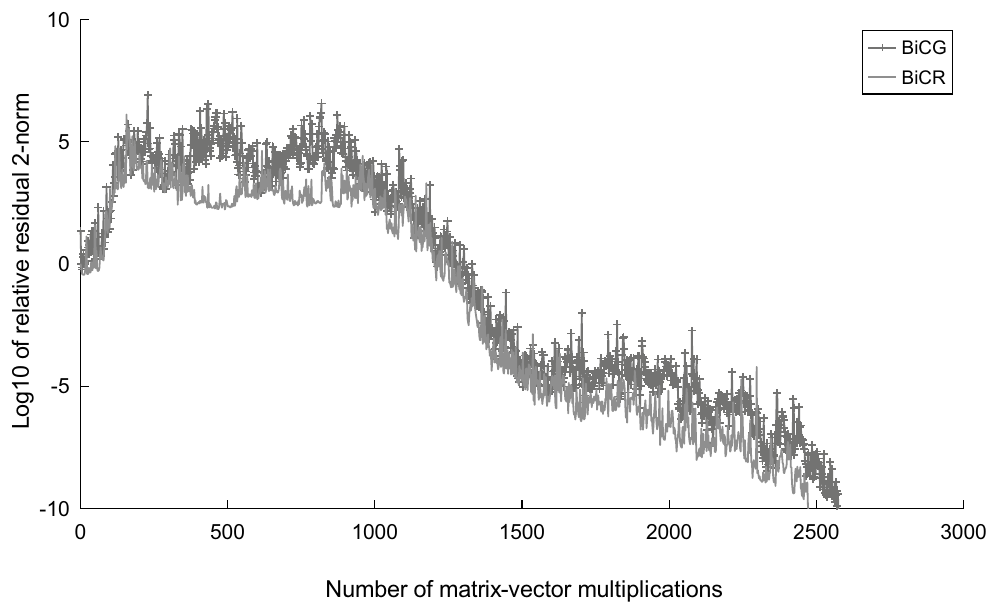
\includegraphics[width=.87\linewidth]{figures/bicg-bicr-far-symmetric.png}
\caption{{当 $b_1=b_2=b_3=10$ 时 BiCG 和 BiCR 的收敛历程}}\label{fig:bicg-bicr-far-symmetric}\end{figure}
% block: qmr-heading pages:121,122 type:subsection
\subsubsection{{准最小残差 (QMR) 方法}}\label{subsec:qmr-method}
{本小节介绍准最小残差 (QMR) 方法 \BookCite{66} 的思想. QMR 方法的推导过程与 Section\ \ref{subsec:qmr-sym} 中 QMR\_SYM 方法的推导过程几乎相同. 主要区别是不采用复对称 Lanczos 过程, 而采用双 Lanczos 过程. 设 $V_n$ 为通过 Algorithm\ \ref{alg:bi-lanczos} 给出的双 Lanczos 过程得到的 $\mathcal K_n(A,\bm r_0)$ 的双正交基. 则 QMR 方法寻找近似解 $\bm x_n$, 使 $\bm x_n$ 位于仿射空间 $\bm x_0+\mathcal K_n(A,\bm r_0)$ 中, 即,}
\[\bm x_n=\bm x_0+V_n\bm y_n,\quad\bm y_n\in\mathbb C^n.\]
{相应的残差向量为}
\[\bm r_n=\bm r_0-AV_n\bm y_n.\]
{由双 Lanczos 过程的矩阵形式 \eqref{eq:bilanczos-matrix-relation} 得}
\[\bm r_n=\bm r_0-V_{n+1}T_{n+1,n}\bm y_n=V_{n+1}(\beta\bm e_1-T_{n+1,n}\bm y_n),\]
{其中 $\beta:=\|\bm r_0\|$. 上述推导过程与 MINRES 方法的推导过程很相似; 然而, 在此情形下, 若选择 $\bm y_n$ 使残差范数达到极小值, 则可能导致如 Section\ \ref{subsec:qmr-sym} 所述的大量计算开销和内存需求. 与 QMR\_SYM 方法类似, QMR 方法选择 $\bm y_n$ 使得}
\begin{equation}\label{eq:qmr-projected-minimization}\bm y_n:=\operatorname*{arg\,min}_{\bm y\in\mathbb C^n}\|\beta\bm e_1-T_{n+1,n}\bm y\|.\end{equation}
{这一极小化问题可由 Givens 旋转高效求解. 按照 \eqref{eq:minres-projected-least-squares} 的求解及 Section\ \ref{subsec:qmr-sym}, 即得到 QMR 方法, 其算法见 Algorithm\ \ref{alg:qmr}.}
% block: qmr-breakdown pages:122,123 type:ordinary-paragraph
{最后应注意, Algorithm\ \ref{alg:qmr} 与 BiCG 方法及 BiCR 方法一样, 存在发生中断 (除以零) 的可能性. 在有限精度运算中, 这样的中断很罕见; 但可能发生近中断, 并导致数值不稳定. 因此, 为避免 (近) 中断问题, \BookCite{66} 中的 QMR 方法使用由 Taylor \BookCite{189} 和 Parlett 等 \BookCite{145} 提出的前瞻 Lanczos 过程.}
% block: qmr-algorithm page:123 type:ordinary-paragraph
\begin{algorithm}[H]\caption{{QMR 方法}}\label{alg:qmr}\begin{algorithmic}[1]
\Statex\textbf{Input:} $\bm x_0\in\mathbb C^N,\ \beta_0=0,\ \gamma_0=0,\ \bm v_0=\bm0,\ \bm w_0=\bm0,\ \bm r_0=\bm b-A\bm x_0$
\Statex\textbf{Output:} $\bm x_n$
\State $\bm g=(\|\bm r_0\|,0,\ldots,0)^{\top},\quad\bm v_1=\bm r_0/\|\bm r_0\|$
\For{$n=1,2,\ldots$}
\State ({双 Lanczos 过程})
\State $\alpha_n=(\bm w_n,A\bm v_n),$
\State $\widetilde{\bm v}_{n+1}=A\bm v_n-\alpha_n\bm v_n-\beta_{n-1}\bm v_{n-1}$
\State $\widetilde{\bm w}_{n+1}=A^{\mathrm H}\bm w_n-\bar\alpha_n\bm w_n-\gamma_{n-1}\bm w_{n-1}$
\State $\gamma_n=\|\widetilde{\bm v}_{n+1}\|_2$
\State $\bm v_{n+1}=\widetilde{\bm v}_{n+1}/\gamma_n$
\State $\beta_n=(\widetilde{\bm w}_{n+1},\bm v_{n+1})$
\State $\bm w_{n+1}=\widetilde{\bm w}_{n+1}/\bar\beta_n$
\State (Givens {旋转})
\State \textbf{for} $i=\max\{1,n-2\},\ldots,n-1$ \textbf{do}
\State $\begin{bmatrix}t_{i,n}\\t_{i+1,n}\end{bmatrix}=\begin{bmatrix}c_i&s_i\\-\bar s_i&c_i\end{bmatrix}\begin{bmatrix}t_{i,n}\\t_{i+1,n}\end{bmatrix}$
\State \textbf{end for}
\State $c_n=\frac{|t_{n,n}|}{\sqrt{|t_{n,n}|^2+|t_{n+1,n}|^2}}$
\State $\bar s_n=\frac{t_{n+1,n}}{t_{n,n}}c_n$
\State $t_{n,n}=c_nt_{n,n}+s_nt_{n+1,n}$
\State $t_{n+1,n}=0$
\State $\begin{bmatrix}g_n\\g_{n+1}\end{bmatrix}=\begin{bmatrix}c_n&s_n\\-\bar s_n&c_n\end{bmatrix}\begin{bmatrix}g_n\\0\end{bmatrix}$
\State ({更新} $\bm x_n$)
\State $\bm p_n=(\bm v_n-t_{n-2,n}\bm p_{n-2},$
\State $\qquad-t_{n-1,n}\bm p_{n-1})/t_{n,n}$
\State $\bm x_n=\bm x_{n-1}+g_n\bm p_n$
\State ({检查收敛})
\State $A\bm p_n=(A\bm v_n-t_{n-2,n}A\bm p_{n-2}$
\State $\qquad-t_{n-1,n}A\bm p_{n-1})/t_{n,n}$
\State $\bm r_n=\bm r_{n-1}-g_nA\bm p_n$
\State {若 $\|\bm r_n\|/\|\bm b\|\le\epsilon$, 则停止}
\EndFor\end{algorithmic}\end{algorithm}
% block: gmres-heading pages:123,124 type:subsection
\subsubsection{{广义最小残差 (GMRES) 方法}}\label{subsec:gmres-method}
{GMRES 方法 \BookCite{152} 的推导过程与 Section\ \ref{subsec:minres} 中的 MINRES 方法密切相关. GMRES 方法生成使 $\|\bm b-A\bm x_n\|$ 在仿射空间 $\bm x_0+\mathcal K_n(A,\bm r_0)$ 上达到极小值的 $\bm x_n$. 这可通过 Section\ \ref{subsec:arnoldi-process} 中的 Arnoldi 过程高效实现. 下面给出 GMRES 方法的推导过程.}
{设 $V_n$ 为 $N$ 行 $n$ 列的矩阵, 其列为 Arnoldi 过程生成的 $\mathcal K_n(A,\bm r_0)$ 的标准正交基向量. 于是, 由于 $\bm x_n$ 位于仿射空间 $\bm x_0+\mathcal K_n(A,\bm r_0)$ 中, 有}
\[\bm x_n=\bm x_0+V_n\bm y_n,\quad\bm y_n\in\mathbb C^n.\]
{相应的残差向量写为}
\[\bm r_n=\bm r_0-AV_n\bm y_n.\]
{由 \eqref{eq:arnoldi-matrix-relation} 中 Arnoldi 过程的矩阵表示得}
\begin{equation}\label{eq:gmres-projected-residual}\bm r_n=V_{n+1}(\beta\bm e_1-H_{n+1,n}\bm y_n),\end{equation}
{其中 $\beta:=\|\bm r_0\|$. 由于 $V_{n+1}^{\mathrm H}V_{n+1}=I_{n+1}$, 即单位矩阵, 残差向量的 2-范数为}
\[\|\bm r_n\|=\|V_{n+1}(\beta\bm e_1-H_{n+1,n}\bm y_n)\|=\|\beta\bm e_1-H_{n+1,n}\bm y_n\|.\]
{因此, 按下式选择 $\bm y_n$ 可使残差向量的 2-范数达到极小值:}
\begin{equation}\label{eq:gmres-projected-minimization}\bm y_n:=\operatorname*{arg\,min}_{\bm y\in\mathbb C^n}\|\beta\bm e_1-H_{n+1,n}\bm y\|.\end{equation}
{向量 $\bm y_n$ 可通过 Givens 旋转得到. 按照 \eqref{eq:minres-projected-least-squares} 的求解就得到 GMRES 方法. 下面在 Algorithm\ \ref{alg:gmres} 中描述 GMRES 算法, 它基于改进 Gram--Schmidt 型 Arnoldi 过程 (Algorithm\ \ref{alg:arnoldi-modified}).}
% block: gmres-algorithm page:124 type:ordinary-paragraph
\begin{algorithm}[H]\caption{{改进 Gram-Schmidt 型 GMRES 方法}}\label{alg:gmres}\begin{algorithmic}[1]
\Statex\textbf{Input:} $\bm x_0\in\mathbb C^N,\ \bm r_0=\bm b-A\bm x_0$
\Statex\textbf{Output:} $\bm x_n$
\State $\bm g=(\|\bm r_0\|,0,\ldots,0)^{\top},\quad\bm v_1=\bm r_0/\|\bm r_0\|$
\For{$n=1,2,\ldots$}
\State (Arnoldi {过程})
\State $\bm t=A\bm v_n$
\For{$i=1,2,\ldots,n$}
\State $h_{i,n}=(\bm v_i,\bm t)$
\State $\bm t=\bm t-h_{i,n}\bm v_i$
\EndFor
\State $h_{n+1,n}=\|\bm t\|$
\State $\bm v_{n+1}=\bm t/h_{n+1,n}$
\State (Givens {旋转})
\For{$i=1,2,\ldots,n-1$}
\State $\begin{bmatrix}h_{i,n}\\h_{i+1,n}\end{bmatrix}=\begin{bmatrix}c_i&s_i\\-\bar s_i&c_i\end{bmatrix}\begin{bmatrix}h_{i,n}\\h_{i+1,n}\end{bmatrix}$
\EndFor
\State $c_n=\frac{|h_{n,n}|}{\sqrt{|h_{n,n}|^2+|h_{n+1,n}|^2}}$
\State $\bar s_n=\frac{h_{n+1,n}}{h_{n,n}}c_n$
\State $h_{n,n}=c_nh_{n,n}+s_nh_{n+1,n}$
\State $h_{n+1,n}=0$
\State $\begin{bmatrix}g_n\\g_{n+1}\end{bmatrix}=\begin{bmatrix}c_n&s_n\\-\bar s_n&c_n\end{bmatrix}\begin{bmatrix}g_n\\0\end{bmatrix}$
\State ({检查收敛})
\If{$|g_{n+1}|/\|\bm b\|\le\epsilon$}
\State $\bm x_n=\bm x_0+V_nH_n^{-1}\bm g$
\EndIf\EndFor\end{algorithmic}\end{algorithm}
% block: gmres-back-substitution page:124 type:ordinary-paragraph
{注意, 在 Algorithm\ \ref{alg:gmres} 第 22 行计算 $\bm c:=H_n^{-1}\bm g$, 对应于求解形如 $H_n\bm c=\bm g$ 的线性方程组. 经过 Givens 旋转后, $H_n$ 不再是 Hessenberg 矩阵, 而变为上三角矩阵. 因此该线性方程组可通过 \eqref{eq:lu-triangular-solves} 所述的回代容易地求解.}
{下面介绍 GMRES 方法的收敛性分析.}
% block: gmres-convergence-proposition pages:124,125 type:proposition
\par\Needspace{3\baselineskip}
\begin{Proposition}\label{prop:gmres-diagonalizable-bound}
{设 $A$ 为 $N$ 行 $N$ 列的可对角化矩阵, 即 $A=X\Lambda X^{-1}$, 其中 $\Lambda=\operatorname{diag}\{\lambda_1,\ldots,\lambda_N\}$, 设 $\bm r_n$ 为 $m$ 步 GMRES 残差向量. 则}
\[\|\bm r_n\|\le\kappa(X)\epsilon_n\|\bm r_0\|,\]
{其中 $\kappa(X)=\|X\|\|X^{-1}\|$, 且}
\[\epsilon^{(n)}=\min_{p\in\mathbb P_n,p(0)=1}\max_{i=1,\ldots,N}|p(\lambda_i)|.\]
{这里 $\mathbb P_m$ 表示所有次数至多为 $m$ 的多项式构成的集合.}
\end{Proposition}
% block: gmres-convergence-proof page:125 type:proof
\begin{Proof}
{GMRES 方法寻找近似解 $\bm x_n$ 使得}
\[\min_{\bm x_n\in\bm x_0+\mathcal K_n(A,\bm r_0)}\|\bm r_n\|.\]
{由于 $\bm r_n\in\mathcal K_{n+1}(A,\bm r_0)$, GMRES 残差向量可写为矩阵多项式形式 $\bm r_n=(I+c_1A+c_2A^2+\cdots+c_nA^n)\bm r_0$, 其中 $c_i$ 通过极小化 $\|\bm r_n\|$ 确定; 等价地, $\bm r_n=p_n^{(\mathrm{opt})}(A)\bm r_0$, 其中 $p_n^{(\mathrm{opt})}(0)=1$, 且 $p_n^{(\mathrm{opt})}$ 通过极小化 $\|\bm r_n\|$ 确定, 即,}
\[\min_{p\in\mathbb P_n,p(0)=1}\|p_n(A)\bm r_0\|.\]
{因此, 对任意 $p\in\mathbb P_n$ 且 $p(0)=1$, 残差 2-范数 $\|\bm r_n\|$ 有如下界}
\[\begin{aligned}\|\bm r_n\|&=\|p_n^{(\mathrm{opt})}(A)\bm r_0\|\\&\le\|p_n(A)\bm r_0\|\\&=\|Xp_n(\Lambda)X^{-1}\bm r_0\|\\&\le\|X\|\|X^{-1}\|\|p_n(\Lambda)\|\|\bm r_0\|\\&=\kappa(X)\max_{i=1,\ldots,N}|p_n(\lambda_i)|\|\bm r_0\|\end{aligned}\]
{由于上述不等式对任意 $p\in\mathbb P_n$ 且 $p(0)=1$ 都成立, 有}
\[\begin{aligned}\|\bm r_n\|&\le\kappa(X)\left(\min_{p\in\mathbb P_n,p(0)=1}\max_{i=1,\ldots,N}|p(\lambda_i)|\right)\|\bm r_0\|\\&=\kappa(X)\epsilon_n\|\bm r_0\|,\end{aligned}\]
{证明完毕.}
\par\nopagebreak[4]
\end{Proof}
% block: gmres-eigenvalue-discussion page:125 type:ordinary-paragraph
{由 Proposition\ \ref{prop:gmres-diagonalizable-bound}, 若 $X$ 的条件数较小, 则 $\epsilon_n$ 的值高度依赖于收敛速度. 进一步, 若 $X$ 的条件数较小且特征值良好聚集, 则 GMRES 方法表现出良好的收敛行为. 若矩阵 $A$ 对称, 则 $X$ 的条件数为 1. 因此 GMRES 方法 (或 MINRES 方法) 的收敛性仅依赖于特征值的分布. 使用 $\epsilon_n$ 的一个上界, 即可不使用全部特征值而估计收敛行为. 详情见 Saad 的优秀著作 \BookCite{151}, 第 206--207 页.}
% block: restarted-gmres-motivation page:126 type:ordinary-paragraph
{GMRES 方法的良好特点在于, 与基于 BiCG 方法和 BiCR 方法的 Krylov 子空间方法不同, GMRES 方法从不发生中断, 残差 2-范数单调下降, 且具有残差 2-范数意义下的最优性. 另一方面, GMRES 方法的一个缺点是其计算开销和内存需求随迭代次数线性增加. 例如, 若迭代次数为 10000, 则需存储一个 $N\times10000$ 矩阵, 而 \eqref{eq:gmres-projected-minimization} 中最小二乘问题的规模为 $10001\times10000$. 为克服这一缺点, 提出了重启的 GMRES 方法, 见 Algorithm\ \ref{alg:gmres-restarted}.}
{记为 GMRES($m$) 的重启 GMRES 方法的思想是, 运行 GMRES 方法直至达到预定最大迭代次数 $m$, 然后以此前 GMRES 方法在第 $m$ 次迭代产生的近似解作为初始猜测, 重新启动 GMRES 方法.}
% block: restarted-gmres-algorithm page:126 type:ordinary-paragraph
\begin{algorithm}[H]\caption{{GMRES($m$) 方法}}\label{alg:gmres-restarted}\begin{algorithmic}[1]
\Statex\textbf{Input:} {初始猜测 $\bm x_0\in\mathbb C^N$ 和重启数 $m$}
\Statex\textbf{Output:} $\bm x_m$
\State{以 $\bm x_0$ 运行 GMRES 方法 (Algorithm\ \ref{alg:gmres}) 的 $m$ 次迭代, 得到 $\bm x_m$.}
\While{{收敛}}
\State{置 $\bm x_0=\bm x_m$.}
\State{以 $\bm x_0$ 运行 GMRES 方法 (Algorithm\ \ref{alg:gmres}) 的 $m$ 次迭代, 得到 $\bm x_m$.}
\EndWhile\end{algorithmic}\end{algorithm}
% block: gmres-restart-frequency page:126 type:ordinary-paragraph
{考虑 GMRES($m$) 方法的重启频率 $m$ 固定的情形. 这意味着反复对线性方程组应用 $m$ 步 GMRES 方法, 直至收敛. 另一方面, 非固定的重启频率是指先运行 GMRES($m_1$), 然后运行 GMRES($m_2$) 方法, GMRES($m_3$) 方法, 如此继续, 直至收敛. 若 $m_1=m_2=\cdots=m$, 则对应于固定的重启频率.}
{文献 \BookCite{117} 及一些作者研究了对 $k=1,2,\ldots$ 确定 $m_k$ 的高效方法, 例如 \BookCite{14}, \BookCite{137}, \BookCite{176}, \BookCite{211}.}
% block: lgmres-augmentation pages:126,127 type:ordinary-paragraph
{\leavevmode\phantomsection\label{idx:chapter-03-section-03:lgmres-augmentation}GMRES 方法的另一个重要发展是增广. 增广有两种途径: 一种利用此前的近似解, 例如 LGMRES 方法 \BookCite{15}; 另一种利用对应于模较小特征值的近似特征向量, 例如 GMRES-E 方法 \BookCite{134}. 下面介绍 LGMRES 方法和 GMRES-E 方法的基本思想.}
{一组 $m$ 次迭代 (例如 Algorithm\ \ref{alg:gmres-restarted} 中第 3 和第 4 行) 称为一个循环, 将 LGMRES 方法在第 $j$ 个循环后的近似解记为 $\bm x_m^{(j)}$. 令 $\bm z^{(k)}:=\bm x_m^{(j-1)}-\bm x_m^{(j-2)}$. 则对给定的 $l$, LGMRES 方法按下列方式寻找近似解:}
\[\bm x_m^{(j)}=\bm x_m^{(j-1)}+q_{m-1}^{(j)}(A)\bm r_m^{(j-1)}+\sum_{k=j-l}^{j-1}\alpha_{j,k}(A)\bm z^{(k)},\]
{其中 $q_{m-1}^{(j)}(A)$ 为 $m-1$ 次多项式, $\alpha_{j,k}(A)$ 为 $k$ 次多项式. 这些多项式通过极小化 $\bm x_m^{(j)}$ 的残差 2-范数确定. 相关算法例如见 \BookCite{13}, \BookCite{103}, \BookCite{104}, \BookCite{106}.}
% block: gmres-e-augmentation page:127 type:ordinary-paragraph
{将 GMRES-E 方法在第 $j$ 个循环后的近似解记为 $\bm x_m^{(j)}$, $\bm p_k^{(j)}$ 为对应于模第 $k$ 小的近似特征值 (调和 Ritz 值) 的近似特征向量 (调和 Ritz 向量). 则对给定的 $p$, GMRES-E 方法按下列方式寻找近似解:}
\[\bm x_m^{(j)}=\bm x_m^{(j-1)}+q_{m-1}^{(j)}(A)\bm r_m^{(j-1)}+\sum_{k=1}^{p}\beta_{j,k}(A)\bm p_k^{(j-1)},\]
{其中 $q_{m-1}^{(j)}(A)$ 为 $m-1$ 次多项式, $\beta_{j,k}(A)$ 为 $k$ 次多项式. 这些多项式通过极小化 $\bm x_m^{(j)}$ 的残差 2-范数确定. 相关算法例如见 \BookCite{11}, \BookCite{135}. 文献 \BookCite{31} 将 LGMRES 方法和 GMRES-E 方法结合, 提出了使用切换控制器的 LGMRES-E 方法. 粗略地说, 切换规则是在收敛良好时选择 LGMRES 方法, 在发现收敛缓慢时选择 GMRES-E 方法.}
{增广并不只用于 GMRES 方法. 事实上, 文献 \BookCite{74}, \BookCite{89}, \BookCite{90} 建立了包括 BiCG 方法, BiCR 方法及其他重要 Krylov 空间方法在内的 Krylov 子空间方法的增广与消去框架.}
% block: gmres-numerical-example pages:127,128 type:ordinary-paragraph
{最后给出 GMRES 方法和 GMRES($m$) 方法的一个数值例子的结果. 考虑非对称线性方程组 \eqref{eq:three-dimensional-difference-system}, 参数为 $N=20$, $a_1=a_2=a_3=1$, $b_1=b_2=b_3=1$, 以及 $c=1$. 结果见 Figure\ \ref{fig:gmres-restarts}, 其中 GMRES 方法和 GMRES($m$) 方法所用的停止准则为 $\|\bm r_n\|/\|\bm b\|\le10^{-10}$, 横轴为矩阵向量乘法的次数.}
{由 Figure\ \ref{fig:gmres-restarts} 可见, GMRES 方法, GMRES(10) 方法和 GMRES(20) 方法的残差 2-范数单调下降, 这有理论保证. 从矩阵向量乘法次数看, GMRES 方法优于重启 GMRES 方法 (GMRES(10), GMRES(20)). 对 GMRES 方法而言, 由于它在 Krylov 子空间上寻找最佳近似解, 所需的矩阵向量乘法次数最少. 另一方面, 如前所述, GMRES 方法的计算开销随迭代次数线性增加. 这意味着, 当所需迭代次数很大时, 矩阵向量乘法可能不再是最耗时的部分. 从 CPU 时间看, GMRES 方法需要 0.39 秒, GMRES(10) 需要 0.31 秒, GMRES(20) 需要 0.26 秒.}\footnote{{代码: GNU Octave 6.2.0 版, 操作系统: macOS Moterey 12.2.1 版, CPU: Apple M1 pro.}}
{因此, 就 CPU 时间而言, GMRES(20) 方法在所有方法中最好, 它平衡了增加的计算开销与所需的迭代次数.}
% block: gmres-restart-figure page:128 type:figure
\begin{figure}[H]\centering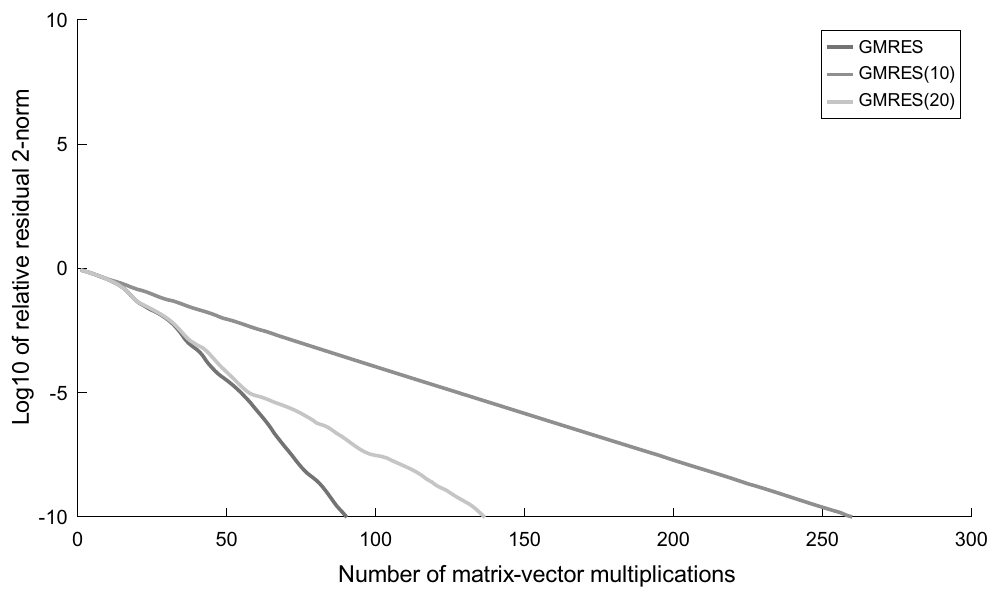
\includegraphics[width=.87\linewidth]{figures/gmres-restarts.png}
\caption{{GMRES, GMRES(10) 和 GMRES(20) 的收敛历程}}\label{fig:gmres-restarts}\end{figure}
% block: gcr-heading pages:128,129 type:subsection
\subsubsection{{广义共轭残差 (GCR) 方法}}\label{subsec:gcr-method}
{广义共轭残差 (GCR) 方法 \BookCite{54} 是另一种基于 Arnoldi 过程的 Krylov 求解器. 在精确运算中, GCR 方法产生与 GMRES 方法相同的近似解. 该算法由下列以 $A^{\mathrm H}A$ 为权且 $\bm r_0=\bm b-A\bm x_0$ 的 Arnoldi 过程得到:}
{置} $\bm v_1=\dfrac{\bm r_0}{\|\bm r_0\|_{A^{\mathrm H}A}}$,\par
{对 $n=1,2,\ldots$, 执行:}
\[h_{i,n}=(\bm v_i,A\bm v_n)_{A^{\mathrm H}A},\quad i=1,2,\ldots,n,\]
\begin{equation}\label{eq:gcr-weighted-arnoldi-remainder}\widetilde{\bm v}_{n+1}=A\bm v_n-\sum_{i=1}^nh_{i,n}\bm v_i,\end{equation}
\[h_{n+1,n}=\|\widetilde{\bm v}_{n+1}\|_{A^{\mathrm H}A},\]
\begin{equation}\label{eq:gcr-weighted-arnoldi-normalization}\bm v_{n+1}=\frac{\widetilde{\bm v}_{n+1}}{h_{n+1,n}}.\end{equation}
{结束}
{该过程生成 $A^{\mathrm H}A$-标准正交向量, 即,}
\[(\bm v_i,A^{\mathrm H}A\bm v_j)=(A\bm v_i,A\bm v_j)=\delta_{i,j}.\]
% block: gcr-residual-expansion page:129 type:ordinary-paragraph
{设 $V_n$ 为以 $\bm v_1,\bm v_2,\ldots,\bm v_n$ 为列的矩阵. 则 GCR 方法生成}
\[\bm x_n=\bm x_0+V_n\bm y_n\]
{使残差 2-范数 $\|\bm r_n\|$ 达到极小值. 相应的残差向量可写为}
\begin{equation}\label{eq:gcr-residual-expansion}\bm r_n=\bm r_0-AV_n\bm y_n=\bm r_0-\sum_{i=1}^ny_iA\bm v_i.\end{equation}
{由上述关系有}
\begin{equation}\label{eq:gcr-residual-basis-update}\bm r_n=\bm r_{n-1}-y_nA\bm v_n.\end{equation}
{未知参数 $y_i$ ($i=1,2,\ldots,n$) 通过极小化残差 2-范数确定, 即由 \eqref{eq:gcr-residual-expansion}, 这可通过下式实现}
\[y_i=(A\bm v_i,\bm r_n),\quad\text{for }i=1,2,\ldots,n.\]
{由于 $A\bm v_i$ 为标准正交向量, 有}
\[y_i=(A\bm v_i,\bm r_0),\quad\text{for }i=1,2,\ldots,n.\]
{这里定义向量 $\bm p_n:=-y_n\widetilde{\bm v}_{n+1}$. 则由 \eqref{eq:gcr-weighted-arnoldi-remainder} 得}
% block: gcr-direction-projection page:130 type:ordinary-paragraph
\begin{equation}\label{eq:gcr-direction-from-arnoldi}\bm p_n=-y_nA\bm v_n-\sum_{i=1}^n(\bm v_i,-y_nA\bm v_n)_{A^{\mathrm H}A}\bm v_i.\end{equation}
{由 \eqref{eq:gcr-residual-basis-update} 有 $-y_nA\bm v_n=\bm r_n-\bm r_{n-1}$. 将此关系代入 \eqref{eq:gcr-direction-from-arnoldi}, 得}
\begin{equation}\label{eq:gcr-direction-residual-difference}\bm p_n=\bm r_n-\bm r_{n-1}-\sum_{i=1}^n(\bm v_i,\bm r_n-\bm r_{n-1})_{A^{\mathrm H}A}\bm v_i\end{equation}
\[=\bm r_n-\sum_{i=1}^n(\bm v_i,\bm r_n)_{A^{\mathrm H}A}\bm v_i-\left(\bm r_{n-1}-\sum_{i=1}^n(\bm v_i,\bm r_{n-1})_{A^{\mathrm H}A}\bm v_i\right).\]
{由于 $\bm r_{n-1}$ 位于 $\mathcal K_n(A,\bm r_0)$ 中, 可展开为 $\bm r_{n-1}=\sum_{i=1}^nc_i\bm v_i$. 于是,}
\[(\bm v_j,\bm r_{n-1})_{A^{\mathrm H}A}=\sum_{i=1}^nc_i(\bm v_j,\bm v_i)=c_i\]
{因为 $(\bm v_j,\bm v_i)=\delta_{j,i}$. 因而有}
\begin{equation}\label{eq:gcr-previous-residual-projection}\bm r_{n-1}=\sum_{i=1}^n(\bm v_i,\bm r_{n-1})_{A^{\mathrm H}A}\bm v_i.\end{equation}
{由 \eqref{eq:gcr-direction-residual-difference} 和 \eqref{eq:gcr-previous-residual-projection}, 向量 $\bm p_n$ 可写为}
\begin{equation}\label{eq:gcr-direction-weighted-projection}\bm p_n=\bm r_n-\sum_{i=1}^n(\bm v_i,\bm r_n)_{A^{\mathrm H}A}\bm v_i.\end{equation}
% block: gcr-normalized-direction page:130 type:ordinary-paragraph
{另一方面, $\bm p_n$ 和 $\bm v_{n+1}$ 的关系为}
\[\bm p_n=-\frac{y_n}{|y_n|}\|A\bm p_n\|\bm v_{n+1},\]
{因为由 $\bm p_n$ 的定义及 \eqref{eq:gcr-weighted-arnoldi-normalization} 得}
\[\begin{aligned}\bm p_n&=-y_n\widetilde{\bm v}_{n+1}\\&=-y_n\|\widetilde{\bm v}_{n+1}\|_{A^{\mathrm H}A}\bm v_{n+1}\\&=-y_n\sqrt{(A\widetilde{\bm v}_{n+1},A\widetilde{\bm v}_{n+1})}\,\bm v_{n+1}\\&=-y_n\sqrt{\left(-\frac1{y_n}A\bm p_n,-\frac1{y_n}A\bm p_n\right)}\,\bm v_{n+1}\\&=-\frac{y_n}{|y_n|}\sqrt{(A\bm p_n,A\bm p_n)}\,\bm v_{n+1}.\end{aligned}\]
% block: gcr-coefficients page:131 type:ordinary-paragraph
{因此, 使用 $\bm v_n=-(|y_{n-1}|/y_{n-1})\times\bm p_{n-1}/\sqrt{(A\bm p_{n-1},A\bm p_{n-1})}$, 有下列关系:}
\[\begin{aligned}y_nA\bm v_n&=(A\bm v_n,\bm r_0)A\bm v_n=\frac{(A\bm p_{n-1},\bm r_0)}{(A\bm p_{n-1},A\bm p_{n-1})}A\bm p_{n-1},\\(\bm v_i,\bm r_n)_{A^{\mathrm H}A}\bm v_i&=\frac{(A\bm p_{i-1},A\bm r_n)}{(A\bm p_{i-1},A\bm p_{i-1})}\bm p_{i-1}.\end{aligned}\]
{因此, 将上述结果代入 \eqref{eq:gcr-residual-basis-update} 和 \eqref{eq:gcr-direction-weighted-projection}, 得}
\[\begin{aligned}\bm r_n&=\bm r_{n-1}-\frac{(A\bm p_{n-1},\bm r_0)}{(A\bm p_{n-1},A\bm p_{n-1})}A\bm p_{n-1},\\\bm p_n&=\bm r_n-\sum_{i=1}^n\frac{(A\bm p_{i-1},A\bm r_n)}{(A\bm p_{i-1},A\bm p_{i-1})}\bm p_{i-1}.\end{aligned}\]
{现在, 由 $\bm p_n$ 的定义, 对某个常数 $c$ 有 $\bm p_{n-1}=c\bm v_n$. 因而 $\bm p_{n-1}$ 与 $\bm v_1,\ldots,\bm v_{n-1}$ 关于 $A^{\mathrm H}A$ 正交. 由 \eqref{eq:gcr-residual-expansion} 得}
\[(A\bm p_{n-1},\bm r_{n-1})=(A\bm p_{n-1},\bm r_0)-\sum_{i=1}^{n-1}y_i(A\bm p_{n-1},A\bm v_i)=(A\bm p_{n-1},\bm r_0).\]
{现在定义 $\alpha_{n-1}$ 和 $\beta_{n-1,i}$ 为}
\begin{equation}\label{eq:gcr-alpha}\alpha_{n-1}=\frac{(A\bm p_{n-1},\bm r_{n-1})}{(A\bm p_{n-1},A\bm p_{n-1})},\end{equation}
\begin{equation}\label{eq:gcr-beta}\beta_{n-1,i}=-\frac{(A\bm p_{i-1},A\bm r_n)}{(A\bm p_{i-1},A\bm p_{i-1})}.\end{equation}
{于是有}
\begin{equation}\label{eq:gcr-residual-recurrence}\bm r_n=\bm r_{n-1}-\alpha_{n-1}A\bm p_{n-1},\end{equation}
\begin{equation}\label{eq:gcr-direction-recurrence}\bm p_n=\bm r_n+\sum_{i=1}^n\beta_{n-1,i}\bm p_{i-1}.\end{equation}
{由残差向量的递推关系得到}
\begin{equation}\label{eq:gcr-solution-recurrence}\bm x_n=\bm x_{n-1}+\alpha_{n-1}\bm p_{n-1}.\end{equation}
{为减少矩阵向量乘法的次数, 使用下列递推式:}
% block: gcr-matvec-recurrence page:132 type:ordinary-paragraph
\begin{equation}\label{eq:gcr-matvec-recurrence}A\bm p_n=A\bm r_n+\sum_{i=1}^n\beta_{n-1,i}A\bm p_{i-1}.\end{equation}
{由 \eqref{eq:gcr-alpha}--\eqref{eq:gcr-matvec-recurrence}, 得到 Algorithm\ \ref{alg:gcr} 中的 GCR 算法.}
% block: gcr-algorithm page:132 type:ordinary-paragraph
\begin{algorithm}[H]\caption{{GCR 方法}}\label{alg:gcr}\begin{algorithmic}[1]
\Statex\textbf{Input:} $\bm x_0\in\mathbb C^N,\ \beta_{-1}=0,\ \bm r_0=\bm b-A\bm x_0,\ \bm p_0=\bm r_0$
\Statex\textbf{Output:} $\bm x_n$
\For{$n=0,1,2,\ldots$, {直至收敛}}
\State $\alpha_n=\frac{(A\bm p_n,\bm r_n)}{(A\bm p_n,A\bm p_n)}$
\State $\bm x_{n+1}=\bm x_n+\alpha_n\bm p_n$
\State $\bm r_{n+1}=\bm r_n-\alpha_nA\bm p_n$
\State $\beta_{n,i}=-\frac{(A\bm p_{i-1},A\bm r_{n+1})}{(A\bm p_{i-1},A\bm p_{i-1})},\quad1\le i\le n+1$
\State $\bm p_{n+1}=\bm r_{n+1}+\sum_{i=1}^{n+1}\beta_{n,i}\bm p_{i-1}$
\State $(A\bm p_{n+1}=A\bm r_{n+1}+\sum_{i=1}^{n+1}\beta_{n,i}A\bm p_{i-1})$
\EndFor\end{algorithmic}\end{algorithm}
% block: gcr-properties-proposition page:132 type:proposition
{下面给出 GCR 方法的性质.}
\par\Needspace{3\baselineskip}
\begin{Proposition}\label{prop:gcr-orthogonality}
{GCR 迭代具有下列性质:}
\begin{enumerate}[label=(G\arabic*),ref=G\arabic*]
\item\label{part:gcr-direction-orthogonality} $(A\bm p_i,A\bm p_j)=0,\quad i\ne j$,
\item $(\bm r_i,A\bm p_j)=0,\quad i>j$,
\item $(\bm r_i,A\bm p_i)=(\bm r_i,A\bm r_i)$,
\item $(\bm r_i,A\bm r_j)=0,\quad i>j$,
\item $(\bm r_i,A\bm p_i)=(\bm r_0,A\bm p_i),\quad i\ge j$.
\end{enumerate}\end{Proposition}
{证明见 \BookCite{54}, Theorem 3.1.}
% block: gcr-restarted-and-orthomin page:132 type:ordinary-paragraph
{由上述性质可见, 前面的推导基于性质 (\ref{part:gcr-direction-orthogonality}). 在精确运算中, GCR 方法和 GMRES 方法一样, 至多在 $N$ 次迭代内收敛. 然而, GCR 方法与 GMRES 方法具有相同的缺点, 即计算工作量和所需内存随迭代次数增加. 因此 \BookCite{54} 提出了称为 GCR($k$) 方法的重启 GCR 版本. 其算法见 Algorithm\ \ref{alg:gcr-restarted}.}
{另一种选择是只保留 $k$ 个方向向量:}
\[\bm p_{n+1}=\bm r_{n+1}+\sum_{i=1}^{\min\{k,n+1\}}\beta_{n,i}\bm p_{i-1}.\]
{这一方法称为 Vinsome \BookCite{201} 提出的 Orthomin 方法. 后来 \BookCite{54} 将 Orthomin 方法称为 \linebreak[4]Orthomin($k$) 方法. Orthomin($k$) 方法的算法见 Algorithm\ \ref{alg:orthomin}.}
% block: gcr-restarted-algorithm page:133 type:ordinary-paragraph
\begin{algorithm}[H]\caption{{GCR($k$) 方法}}\label{alg:gcr-restarted}\begin{algorithmic}[1]
\Statex\textbf{Input:} $\bm x_0\in\mathbb C^N,\ \bm r_0=\bm b-A\bm x_0,\ \bm p_0=\bm r_0$
\Statex\textbf{Output:} $\bm x_{k+1}$
\For{$n=0,1,\ldots,k$ {直至收敛}}
\State $\alpha_n=\frac{(A\bm p_n,\bm r_n)}{(A\bm p_n,A\bm p_n)}$
\State $\bm x_{n+1}=\bm x_n+\alpha_n\bm p_n$
\State $\bm r_{n+1}=\bm r_n-\alpha_nA\bm p_n$
\State $\beta_{n,i}=-\frac{(A\bm p_{i-1},A\bm r_{n+1})}{(A\bm p_{i-1},A\bm p_{i-1})},\quad1\le i\le n+1$
\State $\bm p_{n+1}=\bm r_{n+1}+\sum_{i=1}^{n+1}\beta_{n,i}\bm p_{i-1}$
\State $(A\bm p_{n+1}=A\bm r_{n+1}+\sum_{i=1}^{n+1}\beta_{n,i}A\bm p_{i-1})$
\EndFor\State $\bm x_0=\bm x_{k+1}$\State{重复}
\end{algorithmic}\end{algorithm}
% block: orthomin-algorithm page:133 type:ordinary-paragraph
\begin{algorithm}[H]\caption{{Orthomin($k$) 方法}}\label{alg:orthomin}\begin{algorithmic}[1]
\Statex\textbf{Input:} $\bm x_0\in\mathbb C^N,\ \bm r_0=\bm b-A\bm x_0,\ \bm p_0=\bm r_0$
\Statex\textbf{Output:} $\bm x_n$
\For{$n=0,1,\ldots$, {直至 $\|\bm r_n\|\le\epsilon\|\bm b\|$}}
\State $\alpha_n=\frac{(A\bm p_n,\bm r_n)}{(A\bm p_n,A\bm p_n)}$
\State $\bm x_{n+1}=\bm x_n+\alpha_n\bm p_n$
\State $\bm r_{n+1}=\bm r_n-\alpha_nA\bm p_n$
\State $\beta_{n,i}=-\frac{(A\bm p_{i-1},A\bm r_{n+1})}{(A\bm p_{i-1},A\bm p_{i-1})},\quad n-k+2\le i\le n+1$
\State $\bm p_{n+1}=\bm r_{n+1}+\sum_{i=1}^{\min\{k,n+1\}}\beta_{n,i}\bm p_{i-1}$
\State $(A\bm p_{n+1}=A\bm r_{n+1}+\sum_{i=1}^{n+1}\beta_{n,i}A\bm p_{i-1})$
\EndFor\end{algorithmic}\end{algorithm}
% block: gcr-convergence-proposition pages:133,134 type:proposition
{GCR 方法, GCR($k$) 方法和 Orthomin($k$) 方法的收敛性分析见 Proposition\ \ref{prop:gcr-restarted-convergence}.}
\par\Needspace{3\baselineskip}
\begin{Proposition}\label{prop:gcr-restarted-convergence}
{设 $M$ 为 $A\in\mathbb R^{N\times N}$ 的对称部分, $R$ 为 $A$ 的斜对称部分, 即 $M=(A+A^{\top})/2$, $R=(A-A)^{\top}/2$. 若 $M$ 正定, 则 GCR 方法, GCR($k$) 方法或 Orthomin($k$) 方法生成的残差序列 $\{\bm r_n\}$ 满足}
\[\|\bm r_n\|\le\left(1-\frac{\lambda_{\min}(M)^2}{\lambda_{\max}(A^{\top}A)}\right)^{n/2}\|\bm r_0\|\]
{以及}
\[\|\bm r_n\|\le\left(1-\frac{\lambda_{\min}(M)^2}{\lambda_{\min}(M)\lambda_{\max}(M)+\rho(R)^2}\right)^{n/2}\|\bm r_0\|,\]
{其中 $\lambda_{\min}(M)$ 和 $\lambda_{\max}(M)$ 为对称正定矩阵 $M$ 的最小和最大特征值, $\rho(R)$ 为 $R$ 的谱半径.}
\end{Proposition}
{谱半径见 \eqref{eq:stationary-spectral-radius}. 证明见 \BookCite{54}, Theorem 4.4.}
{由 Proposition\ \ref{prop:gcr-restarted-convergence} 可见, 若 $A$ 接近 $I$, 则这三种方法收敛很快, 因为 $\lambda_{\min}(M)\approx\lambda_{\max}(M)\approx1$ 且 $R\approx O$.}
% block: fom-heading page:134 type:subsection
\subsubsection{{完全正交化方法 (FOM)}}\label{subsec:fom}
{FOM \BookCite{149} 是 CG 方法的推广. 与 CG 方法一样, FOM 寻找满足下列条件的近似解}
\[\begin{aligned}\bm x_n&=\bm x_0+\bm z_n,\quad\bm z_n\in\mathcal K_n(A,\bm r_0),\\\bm r_n&\perp\mathcal K_n(A,\bm r_0).\end{aligned}\]
{FOM 使用 Section\ \ref{subsec:arnoldi-process} 中的 Arnoldi 方法生成 $\mathcal K_n(A,\bm r_0)$ 的标准正交基向量. 因而残差向量 $\bm r_n$ 与 \eqref{eq:gmres-projected-residual} 具有相同的形式, 即,}
\begin{equation}\label{eq:fom-projected-residual}\bm r_n=V_{n+1}(\beta\bm e_1-H_{n+1,n}\bm y_n).\end{equation}
{GMRES 方法与 FOM 的区别在于, GMRES 方法寻找使残差向量的 2-范数 $\|\bm r_n\|$ 达到极小值的 $\bm y_n$, 而 FOM 寻找使残差向量与 $n$ 维 Krylov 子空间正交的 $\bm y_n$, 即 $\bm r_n\perp\mathcal K_n(A,\bm r_0)$. 设 $\bm v_i$ 为 $V_{n+1}$ 的第 $i$ 列. 则}
\[\begin{aligned}V_n^{\mathrm H}\bm r_n=\bm0&\Leftrightarrow\bm v_i^{\mathrm H}\bm r_n=0\quad\text{for }i=1,2,\ldots,n\\&\Leftrightarrow\bm r_n^{\mathrm H}(c_1\bm v_1+c_2\bm v_2+\cdots+c_n\bm v_n)=0\quad\text{for all }c_i\in\mathbb C\\&\Leftrightarrow\bm r_n\perp\mathcal K_n(A,\bm r_0).\end{aligned}\]
% block: fom-projected-solve page:134 type:ordinary-paragraph
{注意, 令 $c_i=1$, 且对 $i\ne j$ 令 $c_j=0$, 就可说明断言 $\bm v_i^{\mathrm H}\bm r_n=0\Leftarrow\bm r_n^{\mathrm H}(c_1\bm v_1+c_2\bm v_2+\cdots+c_n\bm v_n)=0$. 由此, 寻找使 $\bm r_n\perp\mathcal K_n(A,\bm r_0)$ 的 $\bm y_n$, 等价于确定使 $V_n^{\mathrm H}\bm r_n=\bm0$ 的 $\bm y_n$. 于是由 \eqref{eq:fom-projected-residual} 得}
\[\bm0=V_n^{\mathrm H}\bm r_n=V_n^{\mathrm H}V_{n+1}(\beta\bm e_1-H_{n+1,n}\bm y_n)=\beta\bm e_1-H_{n,n}\bm y_n.\]
{因此 $\bm y_n$ 可通过求解下列线性方程组得到:}
\[H_{n,n}\bm y_n=\beta\bm e_1.\]
{由于 $H_{n,n}$ 为 Hessenberg 矩阵, 可通过 LU 分解以 $O(n^2)$ 的计算开销求解该线性方程组. GMRES 方法出现后, FOM 的吸引力有所降低, 因为与 GMRES 方法不同, FOM 可能因使用不选主元的 LU 分解而发生中断. 另一方面, 在考虑重启时, 用 FOM 求解 Chapter\ \ref{chap:shifted-linear-systems} 中的移位线性方程组仍有吸引力.}
% block: product-type-heading page:135 type:subsection
\subsubsection{{乘积型 Krylov 子空间方法}}\label{subsec:product-type-krylov}
{如 Section\ \ref{subsec:bicg-method} 所示, BiCG 方法求解 $A\bm x=\bm b$ 时需要 $A^{\mathrm H}$. P. Sonneveld 发现, 将 BiCG 多项式平方可得到一种不使用 $A^{\mathrm H}$ 信息的算法, 所得算法称为 CGS 方法 \BookCite{173}. 虽然收敛性取决于线性方程组, 但当 BiCG 方法表现出平滑的收敛行为时, CGS 方法比 BiCG 方法快得多. 然而, CGS 方法有时表现出很不规则的收敛, 可能发生近似解精度损失或发散. H. A. van der Vorst 观察到, BiCG 多项式的平方可替换为一次最小残差多项式与 BiCG 多项式的乘积, 由此得到 BiCGSTAB 方法 \BookCite{195}, 它往往比 CGS 方法具有更平滑的收敛行为. M. H. Gutknecht 提出二次最小残差多项式与 BiCG 多项式相乘, 称为 BiCGSTAB2 方法 \BookCite{87}. G. L. G. Sleijpen 和 D. R. Fokkema 提出 $\ell$ 次最小残差多项式与 BiCG 多项式相乘, 称为 BiCGSTAB($\ell$) 方法 \BookCite{162}. S.-L. Zhang 构造了包含 CGS 方法, BiCGSTAB 方法和 BiCGSTAB2 方法的框架. 在这一框架中, 文献 \BookCite{212} 提出了 GPBiCG 方法. 这些方法称为 (基于 Bi-CG 方法的) 乘积型方法, 这一名称首先由 S.-L. Zhang 提出.}
{本节根据 Zhang 的著作 \BookCite{72} 介绍 Zhang 的框架.}
% block: product-bicg-polynomials page:135 type:ordinary-paragraph
{如 \eqref{eq:cg-residual-direction-polynomials} 所示, CG 方法的残差向量可写为 Lanczos 多项式与初始残差向量 $\bm r_0$ 的乘积. 类似地, BiCG 方法的残差向量也可写为}
\[\bm r_n^{\mathrm{BiCG}}=R_n(A)\bm r_0,\]
{其中}
\begin{equation}\label{eq:product-bicg-polynomials-initial}R_0(\lambda)=1,\quad P_0(\lambda)=1,\end{equation}
\begin{equation}\label{eq:product-bicg-residual-polynomial}R_n(\lambda)=R_{n-1}(\lambda)-\alpha_{n-1}\lambda P_{n-1}(\lambda),\end{equation}
\begin{equation}\label{eq:product-bicg-direction-polynomial}P_n(\lambda)=R_n(\lambda)+\beta_{n-1}P_{n-1}(\lambda)\quad n=1,2,\ldots\end{equation}
{CG 方法与 BiCG 方法的 (矩阵) 多项式表示的区别在于 Lanczos 多项式中的 $\alpha_i$ 和 $\beta_i$. 基于 BiCG 方法的乘积型方法的第 $n$ 个残差向量, 定义为 $n$ 次多项式与 BiCG 方法的第 $n$ 个残差向量的乘积, 如下所示:}
\begin{equation}\label{eq:product-residual-polynomial}\bm r_n=H_n(A)\bm r_n^{\mathrm{BiCG}}=H_n(A)R_n(A)\bm r_0.\end{equation}
% block: product-polynomial-restructuring page:136 type:subsection
\paragraph{{残差多项式的重构}}\label{subsec:product-polynomial-restructuring}\mbox{}\par
{S.-L. Zhang 提出将 \eqref{eq:product-residual-polynomial} 中的 $H_n$ 定为下列三项递推关系:}
\begin{equation}\label{eq:product-h-initial}H_0(\lambda):=1,\end{equation}
\begin{equation}\label{eq:product-h-first}H_1(\lambda):=(1-\zeta_0\lambda)H_0(\lambda),\end{equation}
\begin{equation}\label{eq:product-h-three-term}H_n(\lambda):=(1+\eta_{n-1}-\zeta_{n-1}\lambda)H_{n-1}(\lambda)-\eta_{n-1}H_{n-2}(\lambda),\quad n=2,3,\ldots\end{equation}
{可见 $H_n$ 与 Lanczos 多项式 \eqref{eq:cg-polynomial-initial-zero}--\eqref{eq:cg-polynomial-three-term} 相似.}
{下面将 $H_n$ 改写为耦合的两项递推关系的形式. 引入 $G_{n-1}$ 为}
\[G_{n-1}(\lambda):=\frac{H_{n-1}(\lambda)-H_n(\lambda)}{\lambda},\]
{并将 \eqref{eq:product-h-three-term} 改写为}
\[-(H_{n-1}(\lambda)-H_n(\lambda))=-\zeta_{n-1}\lambda H_{n-1}(\lambda)-\eta_{n-1}(H_{n-2}(\lambda)-H_{n-1}(\lambda)).\]
{于是 \eqref{eq:product-h-initial}--\eqref{eq:product-h-three-term} 中的 $H_n(\lambda)$ 可改写为}
\begin{equation}\label{eq:product-coupled-initial}H_0(\lambda)=1,\quad G_0(\lambda)=\zeta_0,\end{equation}
\begin{equation}\label{eq:product-coupled-h}H_n(\lambda)=H_{n-1}(\lambda)-\lambda G_{n-1}(\lambda),\end{equation}
\begin{equation}\label{eq:product-coupled-g}G_n(\lambda)=\zeta_nH_n(\lambda)+\eta_nG_{n-1}(\lambda),\quad n=1,2,\ldots\end{equation}
% block: product-iterate-polynomial-recurrences page:136 type:subsection
\paragraph{{乘积型方法迭代量的递推公式}}\label{subsec:product-iterate-recurrences}\mbox{}\par
{由于 \eqref{eq:product-bicg-polynomials-initial}--\eqref{eq:product-bicg-direction-polynomial} 及 \eqref{eq:product-coupled-initial}--\eqref{eq:product-coupled-g} 已给出 $R_n,P_n,H_n,G_n$ 的递推关系, 可以使用这些递推关系, 由前一个残差向量 $\bm r_n=H_n(A)R_n(A)\bm r_0$ 计算残差向量 $\bm r_{n+1}=H_{n+1}(A)R_{n+1}(A)\bm r_0$. 事实上, $H_{n+1}R_{n+1}$ 可作如下展开:}
\begin{equation}\label{eq:product-polynomial-residual-three}H_{n+1}R_{n+1}=H_nR_{n+1}-\eta_n\lambda G_{n-1}R_{n+1}-\zeta_n\lambda H_nR_{n+1}\end{equation}
\begin{equation}\label{eq:product-polynomial-residual-two}=H_nR_n-\alpha_n\lambda H_nP_n-\lambda G_nR_{n+1},\end{equation}
\begin{equation}\label{eq:product-polynomial-t}H_nR_{n+1}=H_nR_n-\alpha_n\lambda H_nP_n,\end{equation}
\begin{equation}\label{eq:product-polynomial-y}\lambda G_nR_{n+2}=H_nR_{n+1}-H_{n+1}R_{n+1}-\alpha_{n+1}\lambda H_nP_{n+1}+\alpha_{n+1}\lambda H_{n+1}P_{n+1},\end{equation}
\begin{equation}\label{eq:product-polynomial-p}H_{n+1}P_{n+1}=H_{n+1}R_{n+1}+\beta_nH_nP_n-\beta_n\lambda G_nP_n,\end{equation}
\begin{equation}\label{eq:product-polynomial-w}\lambda H_nP_{n+1}=\lambda H_nR_{n+1}+\beta_n\lambda H_nP_n,\end{equation}
\begin{equation}\label{eq:product-polynomial-u}\lambda G_nP_n=\zeta_n\lambda H_nP_n+\eta_n(H_{n-1}R_n-H_nR_n+\beta_{n-1}\lambda G_{n-1}P_{n-1}),\end{equation}
\begin{equation}\label{eq:product-polynomial-z}G_nR_{n+1}=\zeta_nH_nR_n+\eta_nG_{n-1}R_n-\alpha_n\lambda G_nP_n.\end{equation}
% block: product-auxiliary-vector-recurrences page:137 type:ordinary-paragraph
{定义新的辅助向量为}
\[\begin{aligned}\bm t_n&:=H_n(A)\bm r_{n+1}^{\mathrm{BiCG}},&\bm y_n&:=AG_{n-1}(A)\bm r_{n+1}^{\mathrm{BiCG}},\\\bm p_n&:=H_n(A)\bm p_n^{\mathrm{BiCG}},&\bm w_n&:=AH_n(A)\bm p_{n+1}^{\mathrm{BiCG}},\\\bm u_n&:=AG_n(A)\bm p_n^{\mathrm{BiCG}},&\bm z_n&:=G_n(A)\bm r_{n+1}^{\mathrm{BiCG}}.\end{aligned}\]
{则由 \eqref{eq:product-polynomial-residual-three}--\eqref{eq:product-polynomial-z} 有下列递推公式:}
\begin{equation}\label{eq:product-residual-three}\bm r_{n+1}=\bm t_n-\eta_n\bm y_n-\zeta_nA\bm t_n\end{equation}
\begin{equation}\label{eq:product-residual-two}=\bm r_n-\alpha_nA\bm p_n-A\bm z_n,\end{equation}
\begin{equation}\label{eq:product-t}\bm t_n=\bm r_n-\alpha_nA\bm p_n,\end{equation}
\begin{equation}\label{eq:product-y}\bm y_{n+1}=\bm t_n-\bm r_{n+1}-\alpha_{n+1}\bm w_n+\alpha_{n+1}A\bm p_{n+1},\end{equation}
\begin{equation}\label{eq:product-p}\bm p_{n+1}=\bm r_{n+1}+\beta_n(\bm p_n-\bm u_n),\end{equation}
\begin{equation}\label{eq:product-w}\bm w_n=A\bm t_n+\beta_nA\bm p_n,\end{equation}
\begin{equation}\label{eq:product-u}\bm u_n=\zeta_nA\bm p_n+\eta_n(\bm t_{n-1}-\bm r_n+\beta_{n-1}\bm u_{n-1}),\end{equation}
\begin{equation}\label{eq:product-z}\bm z_n=\zeta_n\bm r_n+\eta_n\bm z_{n-1}-\alpha_n\bm u_n.\end{equation}
{针对残差向量和近似解, 给出了两个递推关系 \eqref{eq:product-residual-three} 和 \eqref{eq:product-residual-two}. 第一个递推关系 \eqref{eq:product-residual-three} 将用于确定两个参数 $\zeta_n$ 和 $\eta_n$, 第二个递推关系 \eqref{eq:product-residual-two} 可用于按下式得到近似解:}
\[\bm x_{n+1}=\bm x_n+\alpha_n\bm p_n+\bm z_n.\]
% block: product-alpha-beta page:137 type:subsection
\paragraph{{$\alpha_n$ 和 $\beta_n$ 的计算}}\label{subsec:product-alpha-beta}\mbox{}\par
{由于 $H_n$ 最高次项的系数为 $(-1)^n\prod_{i=0}^{n-1}\zeta_i$, 得到}
\[\begin{aligned}(\bm r_0^{*},\bm r_n)&=(\bar H_n(A^{\mathrm H})\bm r_0^{*},\bm r_n^{\mathrm{BiCG}})=\left((-1)^n\prod_{i=0}^{n-1}\zeta_i\right)((A^{\mathrm H})^n\bm r_0^{*},\bm r_n^{\mathrm{BiCG}}),\\(\bm r_0^{*},A\bm p_n)&=(\bar H_n(A^{\mathrm H})\bm r_0^{*},A\bm p_n^{\mathrm{BiCG}})=\left((-1)^n\prod_{i=0}^{n-1}\zeta_i\right)((A^{\mathrm H})^n\bm r_0^{*},A\bm p_n^{\mathrm{BiCG}}).\end{aligned}\]
{因此由 \eqref{eq:bicg-alpha-shadow-power} 和 \eqref{eq:bicg-beta-shadow-power} 得}
\[\alpha_n=\frac{(\bm r_0^{*},\bm r_n)}{(\bm r_0^{*},A\bm p_n)},\qquad\beta_n=\frac{\alpha_n}{\zeta_n}\times\frac{(\bm r_0^{*},\bm r_{n+1})}{(\bm r_0^{*},\bm r_n)}.\]
% block: product-implementation page:138 type:subsection
\paragraph{{实现细节}}\label{subsec:product-implementation}\mbox{}\par
{通过确定两个参数 $\zeta_n$ 和 $\eta_n$, 可从 Zhang 的框架导出 CGS 方法, BiCGSTAB 方法, BiCGSTAB2 方法和 GPBiCG 方法等 Krylov 子空间方法. 这些 Krylov 子空间方法与参数的关系列于 Table\ \ref{tab:product-parameters}.}
% block: product-parameters-table page:138 type:table
\begin{table}[H]\centering
\caption{{乘积型方法中 $\zeta_n$ 和 $\eta_n$ 的选择}}\label{tab:product-parameters}
\begin{tabular}{l|l}\hline
CGS&$\zeta_n=\alpha_n,\quad\eta_n=\dfrac{\beta_{n-1}}{\alpha_{n-1}}\alpha_n$\\\hline
BiCGSTAB&$\zeta_n=\operatorname*{arg\,min}_{\zeta_n\in\mathbb C}\|\bm r_{n+1}\|,\quad\eta_n=0$\\\hline
GPBiCG&$\{\zeta_n,\eta_n\}=\operatorname*{arg\,min}_{\zeta_n,\eta_n\in\mathbb C}\|\bm r_{n+1}\|$\\\hline
BiCGSTAB2&{偶数次迭代采用 BiCGSTAB 参数}\\
&{奇数次迭代采用 GPBiCG 参数}\\\hline
\end{tabular}\end{table}
% block: cgs-parameter-choice page:138 type:subsection
\paragraph{{CGS 方法的选择}}\label{subsec:cgs-parameter-choice}\mbox{}\par
{在递推关系 \eqref{eq:product-coupled-h} 和 \eqref{eq:product-coupled-g} 中置 $\zeta_n=\alpha_n$ 且 $\eta_n=(\beta_{n-1}/\alpha_{n-1})\alpha_n$, 就得到 CGS 方法, 即多项式 $H_n$ 和 $G_n$ 变为 Lanczos 多项式:}
\[H_n(\lambda)=R_n(\lambda),\qquad G_n(\lambda)=\alpha_nP_n(\lambda).\]
{这一事实得到关系 $\bm p_n-\bm u_n=\bm z_n/\alpha_n$, 因为由辅助向量的定义有}
\[\begin{aligned}\bm p_n-\bm u_n&=H_n(A)P_n(A)\bm r_0-AG_n(A)P_n(A)\bm r_0\\&=R_n(A)P_n(A)\bm r_0-\alpha_nAP_n(A)P_n(A)\bm r_0\\&=(R_n(A)-\alpha_nAP_n(A))P_n(A)\bm r_0\\&=R_{n+1}(A)P_n(A)\bm r_0\\&=P_n(A)R_{n+1}(A)\bm r_0\\&=P_n(A)\bm r_{n+1}^{\mathrm{BiCG}}\\&=\frac1{\alpha_n}\times G_n(A)\bm r_{n+1}^{\mathrm{BiCG}}\\&=\frac1{\alpha_n}\times\bm z_n.\end{aligned}\]
% block: cgs-auxiliary-rewrite page:139 type:ordinary-paragraph
{注意, 由 \eqref{eq:product-residual-two} 和 \eqref{eq:product-t} 有 $\bm t_{n-1}-\bm r_n=A\bm z_{n-1}$. 使用递推公式 \eqref{eq:product-residual-two} 更新 $\bm r_{n+1}$ 后, 在递推公式 \eqref{eq:product-residual-three}--\eqref{eq:product-z} 中就不再需要辅助向量 $\bm t_n,\bm y_n$ 和 $\bm w_n$. 现在引入下列辅助向量:}
\[\widetilde{\bm u}_n:=A^{-1}\bm u_n/\alpha_n,\qquad\widetilde{\bm z}_n:=\bm z_n/\alpha_n,\]
{以代替 $\bm u_n$ 和 $\bm z_n$. 使用关系 $(\bm r_0^{*},A\bm p_n)=(\bm r_0^{*},\bm u_n/\alpha_n)$ 即可得到 CGS 方法, 其算法见 Algorithm\ \ref{alg:cgs}. 这里已将 $\widetilde{\bm u}_n$ 和 $\widetilde{\bm z}_n$ 改写为 $\bm u_n$ 和 $\bm z_n$.}
% block: cgs-algorithm page:139 type:ordinary-paragraph
\begin{algorithm}[H]\caption{{CGS 方法}}\label{alg:cgs}\begin{algorithmic}[1]
\Statex\textbf{Input:} $\bm x_0\in\mathbb C^N,\ \beta_{-1}=0,\ \bm u_{-1}=\bm z_{-1}=\bm0,\ \bm r_0=\bm b-A\bm x_0$
\Statex\textbf{Input:} {选择 $\bm r_0^{*}\in\mathbb C^N$, 例如 $\bm r_0^{*}=\bm r_0$}
\Statex\textbf{Output:} $\bm x_n$
\For{$n=0,1,\ldots$}
\State $\bm p_n=\bm r_n+\beta_{n-1}\bm z_{n-1}$
\State $\bm u_n=\bm p_n+\beta_{n-1}(\bm z_{n-1}+\beta_{n-1}\bm u_{n-1})$
\State $\alpha_n=\frac{(\bm r_0^{*},\bm r_n)}{(\bm r_0^{*},A\bm u_n)}$
\State $\bm z_n=\bm p_n-\alpha_nA\bm u_n$
\State $\bm x_{n+1}=\bm x_n+\alpha_n(\bm p_n+\bm z_n)$
\State $\bm r_{n+1}=\bm r_n-\alpha_nA(\bm p_n+\bm z_n)$
\State $\beta_n=\frac{(\bm r_0^{*},\bm r_{n+1})}{(\bm r_0^{*},\bm r_n)}$
\EndFor\end{algorithmic}\end{algorithm}
{CGS 方法的残差向量写为 $\bm r_{n+1}=R_{n+1}(A)R_{n+1}(A)\bm r_0$. CGS 方法是 (Bi)CG 平方方法的缩写, 名称来自项 $R_{n+1}(A)R_{n+1}(A)$. 由此, 可以预期 CGS 方法的收敛速度为 BiCG 方法的两倍. 另一方面, 当 BiCG 方法像通常那样表现出不规则的收敛行为时, CGS 方法的收敛行为会很不规则, 导致近似解的精度低得多, 或不收敛.}
% block: bicgstab-parameter-choice pages:139,140 type:subsection
\paragraph{{BiCGSTAB 方法的选择}}\label{subsec:bicgstab-parameter-choice}\mbox{}\par
{若选择 $\eta_n=0$, 并选择 $\zeta_n$ 使残差向量的 2-范数 $\|\bm r_{n+1}\|=\|\bm t_n-\zeta_nA\bm t_n\|$ 达到极小值, 就得到 BiCGSTAB 方法. 为实现这一极小化, 选择 $\zeta_n$ 使下列性质成立:}
\[\bm r_{n+1}\perp A\bm t_n,\]
{或者等价地, 由 \eqref{eq:scalar-residual-minimizer} 得}
\[\zeta_n=\frac{\bm t_n^{\mathrm H}A\bm t_n}{(A\bm t_n)^{\mathrm H}(A\bm t_n)}.\]
{由于 $\eta_n=0$, 得到}
\[\bm u_n=\zeta_nA\bm p_n,\qquad\bm z_n=\zeta_n\bm t_n.\]
{BiCGSTAB 方法的算法见 Algorithm\ \ref{alg:bicgstab}.}
{BiCGSTAB 方法是 BiCG 稳定化方法的缩写. 下面说明稳定化的含义. 由于 $\eta_n=0$, \eqref{eq:product-coupled-h} 和 \eqref{eq:product-coupled-g} 中的递推关系化为}
\[H_n(\lambda)=H_{n-1}(\lambda)-\zeta_{n-1}\lambda H_{n-1}(\lambda)=(1-\zeta_{n-1}\lambda)H_{n-1}(\lambda).\]
{这意味着 BiCGSTAB 方法的残差向量为}
\[\bm r_{n+1}=H_{n+1}(A)R_{n+1}(A)\bm r_0=(I-\zeta_nA)\bm r_n^{\mathrm{BiCG}}.\]
{这表明, 由于选择 $\zeta_n$ 使 $\|\bm r_{n+1}\|$ 达到极小值, 可以预期 BiCG 方法的残差向量得到稳定化, 即可以预期 BiCGSTAB 方法比 BiCG 方法具有更平滑的收敛行为.}
% block: bicgstab-algorithm page:140 type:ordinary-paragraph
\begin{algorithm}[H]\caption{{BiCGSTAB 方法}}\label{alg:bicgstab}\begin{algorithmic}[1]
\Statex\textbf{Input:} $\bm x_0\in\mathbb C^N,\ \beta_{-1}=0,\ \bm p_{-1}=\bm0,\ \bm r_0=\bm b-A\bm x_0$
\Statex\textbf{Input:} {选择 $\bm r_0^{*}\in\mathbb C^N$, 例如 $\bm r_0^{*}=\bm r_0$}
\Statex\textbf{Output:} $\bm x_n$
\For{$n=0,1,\ldots$}
\State $\bm p_n=\bm r_n+\beta_{n-1}(\bm p_{n-1}-\zeta_{n-1}A\bm p_{n-1})$
\State $\alpha_n=\frac{(\bm r_0^{*},\bm r_n)}{(\bm r_0^{*},A\bm p_n)}$
\State $\bm t_n=\bm r_n-\alpha_nA\bm p_n$
\State $\zeta_n=\frac{(A\bm t_n,\bm t_n)}{(A\bm t_n,A\bm t_n)}$
\State $\bm x_{n+1}=\bm x_n+\alpha_n\bm p_n+\zeta_n\bm t_n$
\State $\bm r_{n+1}=\bm t_n-\zeta_nA\bm t_n$
\State $\beta_n=\frac{\alpha_n}{\zeta_n}\times\frac{(\bm r_0^{*},\bm r_{n+1})}{(\bm r_0^{*},\bm r_n)}$
\EndFor\end{algorithmic}\end{algorithm}
% block: gpbicg-parameter-choice pages:140,141 type:subsection
\paragraph{{GPBiCG 方法的选择}}\label{subsec:gpbicg-parameter-choice}\mbox{}\par
{对于 GPBiCG 方法, 通过极小化残差向量的 2-范数 $\|\bm r_{n+1}\|=\|\bm t_n-\eta_n\bm y_n-\zeta_nA\bm t_n\|$ 来选择两个参数 $\eta_n$ 和 $\zeta_n$. 下列正交条件可实现这一极小化:}
\[\bm r_{n+1}\perp A\bm t_n,\qquad\bm r_{n+1}\perp\bm y_n,\]
{或者等价地, 在 \eqref{eq:least-squares-decomposition} 和 \eqref{eq:least-squares-minimizer} 中置 $\bm d=\bm t_n$, $M=[\bm y_n,A\bm t_n]$, $\bm x=[\eta_n,\zeta_n]^{\top}$, 得到}
\[\begin{aligned}\zeta_n&=\frac{(\bm y_n,\bm y_n)(A\bm t_n,\bm t_n)-(\bm y_n,\bm t_n)(A\bm t_n,\bm y_n)}{(A\bm t_n,A\bm t_n)(\bm y_n,\bm y_n)-(\bm y_n,A\bm t_n)(A\bm t_n,\bm y_n)},\\\eta_n&=\frac{(A\bm t_n,A\bm t_n)(\bm y_n,\bm t_n)-(\bm y_n,A\bm t_n)(A\bm t_n,\bm t_n)}{(A\bm t_n,A\bm t_n)(\bm y_n,\bm y_n)-(\bm y_n,A\bm t_n)(A\bm t_n,\bm y_n)}.\end{aligned}\]
{GPBiCG 方法的算法见 Algorithm\ \ref{alg:gpbicg}. 注意, GPBiCG 方法使用两个参数 $\zeta_n$ 和 $\eta_n$ 来极小化残差 2-范数, 而 BiCGSTAB 方法使用一个参数 $\zeta_n$ 来极小化残差 2-范数, 且 $\eta_n=0$. 由此, 可以预期 GPBiCG 方法比 BiCGSTAB 方法表现出更平滑的收敛行为.}
% block: gpbicg-algorithm page:141 type:ordinary-paragraph
\begin{algorithm}[H]\caption{{GPBiCG 方法}}\label{alg:gpbicg}\begin{algorithmic}[1]
\Statex\textbf{Input:} $\bm x_0\in\mathbb C^N,\ \beta_{-1}=0,\ \bm p_{-1}=\bm t_{-1}=\bm u_{-1}=\bm w_{-1}=\bm z_{-1}=\bm0,\ \bm r_0=\bm b-A\bm x_0$
\Statex\textbf{Input:} {选择 $\bm r_0^{*}\in\mathbb C^N$, 例如 $\bm r_0^{*}=\bm r_0$}
\Statex\textbf{Output:} $\bm x_n$
\For{$n=0,1,\ldots$}
\State $\bm p_n=\bm r_n+\beta_{n-1}(\bm p_{n-1}-\bm u_{n-1})$
\State $\alpha_n=\frac{(\bm r_0^{*},\bm r_n)}{(\bm r_0^{*},A\bm p_n)}$
\State $\bm y_n=\bm t_{n-1}-\bm r_n-\alpha_n\bm w_{n-1}+\alpha_nA\bm p_n$
\State $\bm t_n=\bm r_n-\alpha_nA\bm p_n$
\State $\zeta_n=\frac{(\bm y_n,\bm y_n)(A\bm t_n,\bm t_n)-(\bm y_n,\bm t_n)(A\bm t_n,\bm y_n)}{(A\bm t_n,A\bm t_n)(\bm y_n,\bm y_n)-(\bm y_n,A\bm t_n)(A\bm t_n,\bm y_n)}$
\State $\eta_n=\frac{(A\bm t_n,A\bm t_n)(\bm y_n,\bm t_n)-(\bm y_n,A\bm t_n)(A\bm t_n,\bm t_n)}{(A\bm t_n,A\bm t_n)(\bm y_n,\bm y_n)-(\bm y_n,A\bm t_n)(A\bm t_n,\bm y_n)}$
\If{$n=0$}
\State $\zeta_n=\frac{(A\bm t_n,\bm t_n)}{(A\bm t_n,A\bm t_n)},\quad\eta_n=0$
\EndIf
\State $\bm u_n=\zeta_nA\bm p_n+\eta_n(\bm t_{n-1}-\bm r_n+\beta_{n-1}\bm u_{n-1})$
\State $\bm z_n=\zeta_n\bm r_n+\eta_n\bm z_{n-1}-\alpha_n\bm u_n$
\State $\bm x_{n+1}=\bm x_n+\alpha_n\bm p_n+\bm z_n$
\State $\bm r_{n+1}=\bm t_n-\eta_n\bm y_n-\zeta_nA\bm t_n$
\State $\beta_n=\frac{\alpha_n}{\zeta_n}\times\frac{(\bm r_0^{*},\bm r_{n+1})}{(\bm r_0^{*},\bm r_n)}$
\State $\bm w_n=A\bm t_n+\beta_nA\bm p_n$
\EndFor\end{algorithmic}\end{algorithm}
{Fujino \BookCite{71} 从 Zhang 的框架提出 GPBiCG($m,\ell$) 方法. K. Aihara \BookCite{4} 提出了 GPBiCG 方法和 BiCGSTAB($\ell$) 方法的统一推广, 称为 GPBiCGstab($L$) 方法.}
% block: product-numerical-examples page:142 type:subsection
\paragraph{{数值例子}}\label{subsec:product-numerical-examples}\mbox{}\par
{本小节给出一些说明性的数值例子. 考虑非对称线性方程组 \eqref{eq:three-dimensional-difference-system}, 参数为 $N=20$, $a_1=a_2=a_3=1$, $b_1=b_2=b_3=1$, 以及两个不同参数 $c=300$ 和 $c=900$. 所有 Krylov 子空间方法均采用停止准则 $\|\bm r_n\|/\|\bm b\|\le10^{-10}$.}
{当 $c=300$ 时, CGS 方法, BiCGSTAB 方法和 GPBiCG 方法的收敛历程见 Figure\ \ref{fig:product-methods-moderate}. 横轴不是迭代次数, 而是矩阵向量乘法的次数. (CGS 方法, BiCGSTAB 方法和 GPBiCG 方法每次迭代均需两次矩阵向量乘法.)}
{由 Figure\ \ref{fig:product-methods-moderate}, GPBiCG 方法比 BiCGSTAB 方法收敛更快, 而从矩阵向量乘法次数, 或等价的迭代次数看, CGS 方法最好. 另一方面, CGS 方法表现出不规则的收敛行为, 这可能导致精度损失. GPBiCG 方法和 BiCGSTAB 方法表现出相对平滑的收敛行为, 这可能由残差 2-范数的局部极小化所致. 从精度看, CGS 方法, BiCGSTAB 方法和 GPBiCG 方法的真实相对残差 2-范数的 $\log_{10}$ 分别为 $-9.79$, $-10.50$, $-10.17$. 由此, 所有方法都产生了足够精确的近似解.}
% block: product-residual-gap pages:142,143 type:ordinary-paragraph
{\leavevmode\phantomsection\label{idx:chapter-03-section-03:product-residual-gap}接着, $c=900$ 时的收敛历程见 Figure\ \ref{fig:product-methods-difficult}. 由 Figure\ \ref{fig:product-methods-difficult} 可见, CGS 方法表现出很不规则的收敛行为, 收敛也最慢; 从矩阵向量乘法次数看, GPBiCG 方法最好. 从精度看, CGS 方法, BiCGSTAB 方法和 GPBiCG 方法的真实相对残差 2-范数的 $\log_{10}$ 分别为 $-6.37$, $-10.03$, $-9.79$. 这意味着 CGS 方法损失了约四位精度. 这种精度损失称为残差间隙. 因此, 强烈建议在满足停止准则后检查真实相对残差 2-范数, 即 $\|\bm b-A\bm x_n\|/\|\bm b\|$ (不是 $\|\bm r_n\|/\|\bm b\|$!).}
% block: product-moderate-figure page:142 type:figure
\begin{figure}[H]\centering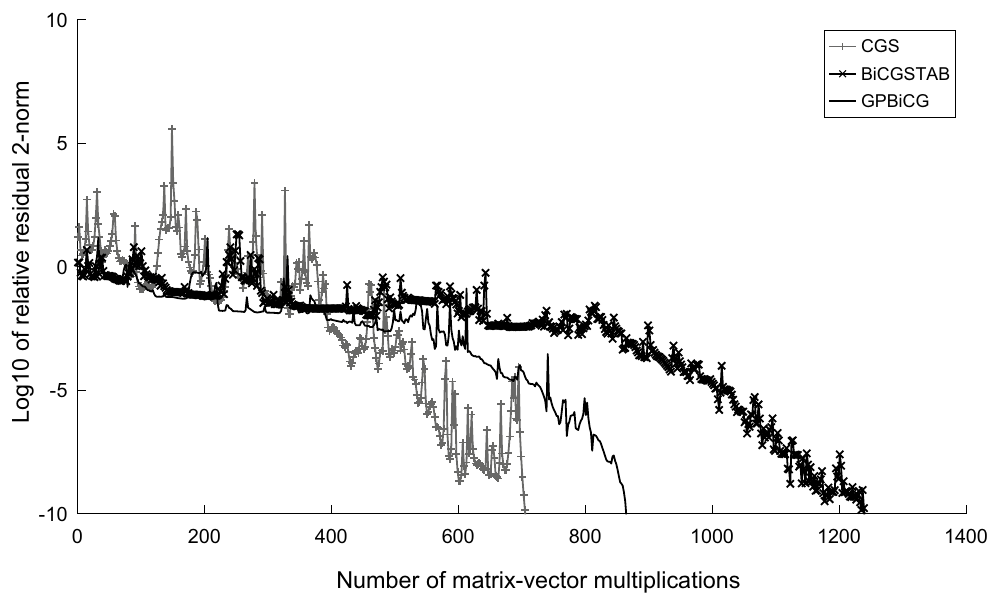
\includegraphics[width=.87\linewidth]{figures/product-methods-moderate.png}
\caption{{当 $N=20,c=300$ 时 CGS, BiCGSTAB 和 GPBiCG 的收敛历程}}\label{fig:product-methods-moderate}\end{figure}
% block: product-difficult-figure page:143 type:figure
\begin{figure}[H]\centering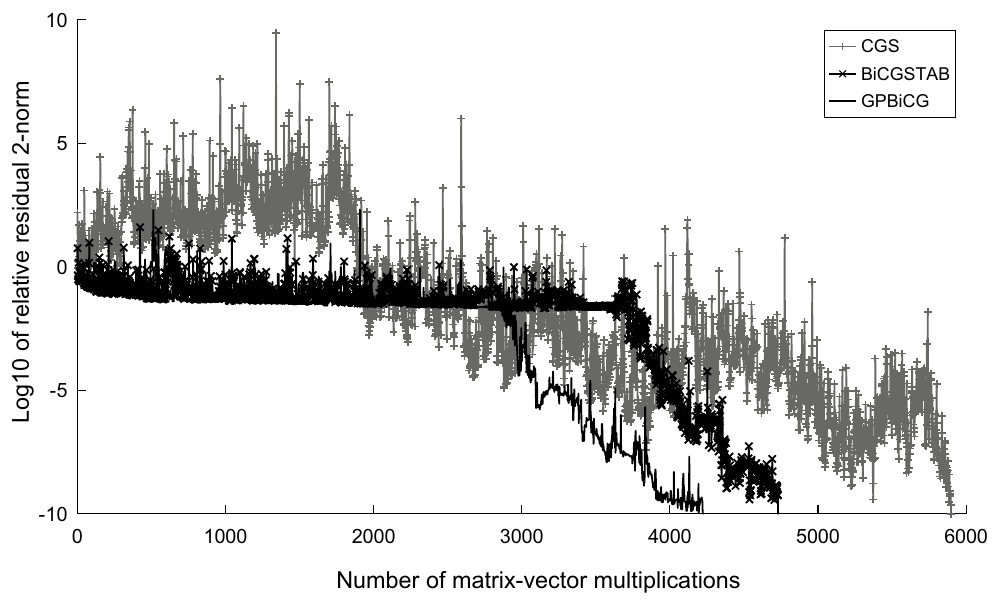
\includegraphics[width=.87\linewidth]{figures/product-methods-difficult.png}
\caption{{当 $N=20,c=900$ 时 CGS, BiCGSTAB 和 GPBiCG 的收敛历程}}\label{fig:product-methods-difficult}\end{figure}
% block: product-related-methods pages:143,144 type:subsection
\paragraph{{其他相关方法}}\label{subsec:product-related-methods}\mbox{}\par
{Section\ \ref{subsec:qmr-method} 中的 QMR 方法与 BiCG 方法一样需要 $A^{\mathrm H}$ 的信息. 与 CGS 方法的思想类似, R. W. Freund 提出了 QMR 方法的平方变型, 称为 TFQMR (无转置 QMR) 方法 \BookCite{63}, 它往往表现出平滑的收敛行为. 文献 \BookCite{34} 基于 BiCGSTAB 方法和 QMR 方法的思想提出 QMRCGSTAB 方法.}
{当系数矩阵 $A$ 接近 Hermitian 矩阵时, Section\ \ref{subsec:bicr-method} 中的 BiCR 方法可能比 BiCG 方法表现出更平滑的收敛行为, 因为当 $A$ 为 Hermitian 矩阵时, 选择 $\bm r_0^{*}=\bm r_0$ 的 BiCR 方法变为 CR 方法, 而 CR 方法的残差 2-范数单调下降. 因此, 自然可以将基于 BiCG 方法的乘积型 Krylov 子空间方法替换为基于 BiCR 方法的乘积型方法. 事实上, 可构造基于 BiCR 方法的乘积型方法, 文献 \BookCite{165} 导出了所得算法 (CRS, BiCRSTAB, GPBiCR). K. Abe 和 G. L. G. Sleijpen 独立提出了基于 BiCR 方法的乘积型方法, 见 \BookCite{2}.}
{Y.-F. Jing 等提出了类似于 BiCR 方法的一种途径, 称为 BiCOR 方法 \BookCite{114}, 其乘积型变型见 \BookCite{32}.}
% block: idr-heading page:144 type:subsection
\subsubsection{{诱导降维 (IDR($s$)) 方法}}\label{subsec:idr-method}
{诱导降维 (IDR) 方法由 Wesseling 和 Sonneveld 于 1979 年前后建立 \BookCite{205}. IDR 方法在数学上等价于 BiCGSTAB 方法, 而 BiCGSTAB 方法可视为 IDR 方法的稳定化变型. 文献 \BookCite{195} 的致谢中写道, Sonneveld 建议 van der Vorst 重新考虑 Sonneveld 的 IDR.}
{虽然 IDR 方法未受到进一步关注, 但大约 30 年后, Sonneveld 和 van Gijzen 提出了一种称为 IDR($s$) 方法的创新算法 \BookCite{174}. 本节介绍 IDR($s$) 方法的理论与推导. 本节推导看似冗长, 但使 IDR($s$) 方法的原理更易理解.}
% block: idr-theorem page:144 type:theorem
\par\Needspace{14\baselineskip}
\begin{Theorem}[{IDR 定理} \BookCite{174}, \BookCite{205}, p.550]\label{thm:idr-dimension-reduction}
{设 $A$ 为 $\mathbb C^{N\times N}$ 中的任意矩阵, $\bm v_0$ 为 $\mathbb C^N$ 中的任意非零向量, $\mathcal G_0$ 为完全 Krylov 空间, 即 $\mathcal G_0:=\mathcal K_N(A,\bm v_0)$. 设 $\mathcal S$ 表示 $\mathbb C^N$ 的任意 (真) 子空间, 使 $\mathcal S$ 和 $\mathcal G_0$ 不具有共同的非平凡不变子空间,}\footnote{{这意味着 $\mathcal S\cap\mathcal G_0$ 不包含 $A$ 的任何特征向量, 平凡不变子空间为 $\{\bm0\}$.}}
{并定义序列 $\mathcal G_j$, $j=1,2,\ldots$ 为}
\begin{equation}\label{eq:idr-subspace-recurrence}\mathcal G_j=(I-\omega_jA)(\mathcal G_{j-1}\cap\mathcal S),\end{equation}
{其中 $\omega_j$ 为非零标量. 则:}
\begin{enumerate}[label=(\arabic*)]
\item $\mathcal G_j\subset\mathcal G_{j-1}$ {对所有 $j>0$ 成立.}
\item $\mathcal G_j=\{\bm0\}$ {对某个 $j\le N$ 成立.}
\end{enumerate}\end{Theorem}
% block: idr-theorem-proof-nesting pages:144,145 type:proof
\begin{Proof}
{本证明基于 \BookCite{174}, Theorem 2.1.}
{第一个断言用归纳法证明. 首先证明 $\mathcal G_1\subset\mathcal G_0$. 由 $\mathcal G_0=\mathcal K_N(A,\bm v_0)$ 得 $(I-\omega_1A)\mathcal G_0\subset\mathcal G_0$, 因为对给定的 $\bm v\in(I-\omega_1A)\mathcal G_0$, 有}
\[\begin{aligned}\bm v&=(I-\omega_1A)(c_0\bm v_0+c_1A\bm v_0+\cdots+c_{N-1}A^{N-1}\bm v_0)\\&=c_0(I-\omega_1A)\bm v_0+c_1(I-\omega_1A)A\bm v_0+\cdots+c_{N-1}(I-\omega_1A)A^{N-1}\bm v_0\\&=d_0\bm v_0+d_1A\bm v_0+\cdots+d_{N-1}A^{N-1}\bm v_0+d_NA^N\bm v_0\\&=\widetilde d_0\bm v_0+\widetilde d_1A\bm v_0+\cdots+\widetilde d_{N-1}A^{N-1}\bm v_0\\&\in\mathcal G_0.\end{aligned}\]
{因此有 $\mathcal G_1\subset\mathcal G_0$, 因为}
\[\mathcal G_1=(I-\omega_1A)(\mathcal G_0\cap\mathcal S)\subset(I-\omega_1A)\mathcal G_0\subset\mathcal G_0.\]
{接着, 在假设 $\mathcal G_j\subset\mathcal G_{j-1}$ 下, 对所有 $j>0$ 证明 $\mathcal G_{j+1}\subset\mathcal G_j$ (即 $\bm x\in\mathcal G_{j+1}\Rightarrow\bm x\in\mathcal G_j$). 设 $\bm x\in\mathcal G_{j+1}$. 则对某个 $\bm y\in\mathcal G_j\cap\mathcal S$, $\bm x$ 可写为 $\bm x=(I-\omega_{j+1}A)\bm y$. 由假设 $\mathcal G_j\subset\mathcal G_{j-1}$, 得 $\bm y\in\mathcal G_j\cap\mathcal S\subset\mathcal G_{j-1}\cap\mathcal S$, 因而 $(I-\omega_jA)\bm y\in\mathcal G_j$. 由于 $\bm y\in\mathcal G_j$ 且 $\bm y-\omega_jA\bm y\in\mathcal G_j$, 有 $A\bm y\in\mathcal G_j$, 从而 $(I-\omega_{j+1}A)\bm y=\bm x\in\mathcal G_j$.}
% block: idr-theorem-proof-dimension page:145 type:proof
{下面证明第二个断言. 性质 $\mathcal G_{j+1}\subset\mathcal G_j$ 意味着 $\dim(\mathcal G_{j+1})<\dim(\mathcal G_j)$ 或 $\dim(\mathcal G_{j+1})=\dim(\mathcal G_j)$.}
{若 $\mathcal G_j\cap\mathcal S\ne\mathcal G_j$, 则 $\dim(\mathcal G_j\cap\mathcal S)<\dim(\mathcal G_j)$, 从而有 $\dim(\mathcal G_{j+1})<\dim(\mathcal G_j)$, 因为 $\dim(\mathcal G_{j+1})=\dim((I-\omega_jA)(\mathcal G_j\cap\mathcal S))\le\dim(\mathcal G_j\cap\mathcal S)<\dim(\mathcal G_j)$.}
{另一方面, 若 $\mathcal G_j\cap\mathcal S=\mathcal G_j$, 则 $\mathcal G_j\subset\mathcal S$, 且有 $\mathcal G_{j+1}=(I-\omega_{j+1}A)(\mathcal G_j\cap\mathcal S)=(I-\omega_{j+1}A)\mathcal G_j\subset\mathcal G_j$. (最后一个包含关系来自第一个断言 $\mathcal G_{j+1}\subset\mathcal G_j$.) 这表明 $A\mathcal G_j\subset\mathcal G_j$, 即 $\mathcal G_j$ 为 $A$ 的不变子空间. 回顾 $\mathcal G_j\subset\mathcal S$ 和 $\mathcal G_j\subset\mathcal G_0$, 得 $\mathcal G_j\subset\mathcal G_0\cap\mathcal S$. 由 $\mathcal G_0\cap\mathcal S$ 不具有共同的 $A$ 的非平凡不变子空间这一假设, 子空间 $\mathcal G_j$ 为 $A$ 的平凡不变子空间, 即 $\mathcal G_j=\{\bm0\}$.}
{因此, 或者 $\dim(\mathcal G_{j+1})<\dim(\mathcal G_j)$, 或者 $\dim(\mathcal G_j)=0$, 这表明对某个 $k\le N$ 有 $\dim(\mathcal G_k)=0$, 即 $\mathcal G_k=\{\bm0\}$.}
\par\nopagebreak[4]
\end{Proof}
% block: idr-dimension-corollary page:145 type:corollary
\par\Needspace{3\baselineskip}
\begin{Corollary}\label{cor:idr-dimension-step}
{对给定的 $s\ge1$, 设 $\mathcal S$ 为 $\mathbb C^N$ 的子空间且 $\dim(\mathcal S)=N-s$. 若 $\mathcal G_{i-1}+\mathcal S=\mathbb C^N$ 且 $(I-\omega_jA)$ 非奇异, 则}
\begin{equation}\label{eq:idr-dimension-step}\dim(\mathcal G_j)=\dim(\mathcal G_{j-1})-s.\end{equation}
\end{Corollary}
% block: idr-dimension-corollary-proof page:145 type:proof
\begin{Proof}
{设 $W_1,W_2$ 为 $\mathbb C^N$ (或一般向量空间 $V$) 的子空间. 线性代数中众所周知, $\dim(W_1)+\dim(W_2)=\dim(W_1+W_2)+\dim(W_1\cap W_2)$. 令 $W_1=\mathcal G_{i-1}$, $W_2=\mathcal S$. 则由假设 $\mathcal G_{i-1}+\mathcal S=\mathbb C^N$, 有 $\dim(\mathcal G_{i-1}+\mathcal S)=N$. 因而 $\dim(\mathcal G_i)=\dim((I-\omega_jA)(\mathcal G_{i-1}\cap\mathcal S))=\dim(\mathcal G_{i-1}\cap\mathcal S)=\dim(\mathcal G_{i-1})+\dim(\mathcal S)-N=\dim(\mathcal G_{i-1})-s$.}
\par\nopagebreak[4]
\end{Proof}
% block: idr-dimension-remark page:145 type:remark
\par\Needspace{3\baselineskip}
\begin{Remark}\label{rem:idr-dimension-count}
{由 Corollary\ \ref{cor:idr-dimension-step}, 若对 $i=1,2,\ldots,n$ 有 $\mathcal G_{i-1}+\mathcal S=\mathbb C^N$, 则 $\dim(\mathcal G_n)=\dim(\mathcal G_0)-ns$. 因而, 若 $N/s$ 为整数且 $\dim(\mathcal G_0)=N$, 则有 $\dim(\mathcal G_{N/s})=0$, 即 $\mathcal G_{N/s}=\{\bm0\}$. Remark\ \ref{rem:idr-matvec-bound} 将引用本注以给出 IDR($s$) 方法所需矩阵向量乘法次数的最大值.}
\end{Remark}
% block: idr-derivation-heading pages:145,146 type:subsection
\paragraph{{IDR($s$) 方法的推导}}\label{subsec:idr-derivation}\mbox{}\par
{对于给定数 $s\ge1$, IDR($s$) 方法生成满足下列条件的残差向量 $\bm r_0,\bm r_1,\ldots$:}
\begin{enumerate}
\item $\bm r_{j(s+1)},\bm r_{j(s+1)+1},\ldots,\bm r_{j(s+1)+s}\in\mathcal G_j,\quad j=0,1,2,\ldots$;
\item{选择 \eqref{eq:idr-subspace-recurrence} 中的子空间 $\mathcal S$, 使 $\dim\mathcal S=N-s$.}
\end{enumerate}
{为简单起见, 考虑 $s=2$ 的情形, 即 IDR(2) 方法. 在此情形下, IDR(2) 方法产生下列残差向量:}
\[\bm r_0,\bm r_1,\bm r_2\in\mathcal G_0,\quad\bm r_3,\bm r_4,\bm r_5\in\mathcal G_1,\quad\bm r_6,\bm r_7,\bm r_8\in\mathcal G_2,\ldots\]
% block: idr-two-shadow-space page:146 type:ordinary-paragraph
{这里说明如何从给定残差向量 $\bm r_0,\bm r_1,\bm r_2\in\mathcal G_0$ 产生 $\bm r_3,\bm r_4,\bm r_5\in\mathcal G_1$. 由于 $s=2$, 由 Remark\ \ref{rem:idr-dimension-count} 可知, 需选择 $\mathcal S$ 使 $\dim(\mathcal S)=N-2$. 标准选择为}
\begin{equation}\label{eq:idr-shadow-complement}\mathcal S=\operatorname{span}\{\bm s_1,\bm s_2\}^{\perp}\end{equation}
{其中 $\bm s_1$ 和 $\bm s_2$ 为任意线性无关向量, 符号 $\perp$ 表示正交补.}
{现在令 $S=[\bm s_1,\bm s_2]\in\mathbb C^{N\times2}$, 其中向量 $\bm s_1$ 和 $\bm s_2$ 线性无关. 则对于向量 $\bm v\in\mathbb C^N$, 下列事实成立:}
\begin{equation}\label{eq:idr-shadow-orthogonality}\bm v\perp\mathcal S\Leftrightarrow S^{\mathrm H}\bm v=\bm0.\end{equation}
{下面使用下列定义:}
\begin{equation}\label{eq:idr-residual-differences}\Delta\bm r_k:=\bm r_{k+1}-\bm r_k,\quad dR_k:=[\Delta\bm r_k,\Delta\bm r_{k+1}],\quad\bm c_k=(S^{\mathrm H}dR_k)^{-1}S^{\mathrm H}\bm r_{k+2}.\end{equation}
% block: idr-first-subspace-residuals pages:146,147 type:ordinary-paragraph
{下列向量 $\bm v_0$ 位于 $\mathcal G_0\cap\mathcal S$ 中:}
\begin{equation}\label{eq:idr-first-projected-vector}\bm v_0=\bm r_2-dR_0\bm c_0\in\mathcal G_0\cap\mathcal S.\end{equation}
{事实上, $\bm v_0\in\mathcal G_0$, 因为 $\bm v_0\in\operatorname{span}\{\bm r_2,\Delta\bm r_0,\Delta\bm r_1\}$, 而由假设 $\bm r_0,\bm r_1,\bm r_2\in\mathcal G_0$ 有 $\bm r_2,\Delta\bm r_0,\Delta\bm r_1\in\mathcal G_0$; 又有 $\bm v_0\in\mathcal S$, 因为容易看出 $S^{\mathrm H}\bm v_0=\bm0$, 并使用关系 \eqref{eq:idr-shadow-orthogonality}.}
{由 \eqref{eq:idr-subspace-recurrence}, 可按下式产生 $\bm r_3\in\mathcal G_1$}
\begin{equation}\label{eq:idr-first-reduced-residual}\bm r_3=(I-\omega_0A)\bm v_0\in\mathcal G_1,\end{equation}
{其中通常选择 $\omega_0$ 使 $\|\bm r_3\|$ 达到极小值, 即 $\omega_0=(A\bm v_0,\bm v_0)/(A\bm v_0,A\bm v_0)$.}
{为产生 $\bm r_4\in\mathcal G_1$, 需要一个使 $\bm v_1\in\mathcal G_0\cap\mathcal S$ 的向量 $\bm v_1$. 为此, 利用 $\bm r_3$ 和 $dR_1$ 按下式构造 $\bm v_1$:}
\[\bm v_1=\bm r_3-dR_1\bm c_1\in\mathcal G_0\cap\mathcal S.\]
{由与上面类似的讨论, 可见 $\bm v_1\in\mathcal G_0$ 且 $\bm v_1\in\mathcal S$. 因此有}
\[\bm r_4=(I-\omega_0A)\bm v_1\in\mathcal G_1.\]
{类似地,}
\[\bm v_2=\bm r_4-dR_2\bm c_2\in\mathcal G_0\cap\mathcal S,\quad\bm r_5=(I-\omega_0A)\bm v_2\in\mathcal G_1.\]
% block: idr-second-subspace-residuals page:147 type:ordinary-paragraph
{现在, 已从给定残差向量 $\bm r_0,\bm r_1,\bm r_2\in\mathcal G_0$ 得到 $\bm r_3,\bm r_4,\bm r_5\in\mathcal G_1$. 类似地, 下列算法从 $\bm r_3,\bm r_4,\bm r_5\in\mathcal G_1$ 产生 $\bm r_6,\bm r_7,\bm r_8\in\mathcal G_2$:}
\[\begin{aligned}\bm v_3&=\bm r_5-dR_3\bm c_3\in\mathcal G_1\cap\mathcal S,&\bm r_6&=(I-\omega_1A)\bm v_3\in\mathcal G_2,\\\bm v_4&=\bm r_6-dR_4\bm c_4\in\mathcal G_1\cap\mathcal S,&\bm r_7&=(I-\omega_1A)\bm v_4\in\mathcal G_2,\\\bm v_5&=\bm r_7-dR_5\bm c_5\in\mathcal G_1\cap\mathcal S,&\bm r_8&=(I-\omega_1A)\bm v_5\in\mathcal G_2,\end{aligned}\]
{其中通常选择 $\omega_1$ 使 $\|\bm r_6\|$ 达到极小值, 即 $\omega_1=(A\bm v_3,\bm v_3)/(A\bm v_3,A\bm v_3)$.}
% block: idr-solution-extraction page:147 type:ordinary-paragraph
{现在说明如何从 $\bm x_0,\bm x_1,\bm x_2$ 提取近似解 $\bm x_3,\bm x_4,\bm x_5$. 下面使用下列定义:}
\[\Delta\bm x_k:=\bm x_{k+1}-\bm x_k,\qquad dX_k:=[\Delta\bm x_k,\Delta\bm x_{k+1}].\]
{于是由 \eqref{eq:idr-first-projected-vector} 和 \eqref{eq:idr-first-reduced-residual}, 按下式得到 $\bm x_3$:}
\[\begin{aligned}\bm r_3&=(I-\omega_0A)\bm v_0=\bm r_2-dR_0\bm c_0-\omega_0A\bm v_0\\&\Leftrightarrow\bm b-A\bm x_3=\bm b-A\bm x_2-dR_0\bm c_0-\omega_0A\bm v_0\\&\Leftrightarrow\bm x_3=\bm x_2+A^{-1}dR_0\bm c_0+\omega_0\bm v_0\\&\Leftrightarrow\bm x_3=\bm x_2-dX_0\bm c_0+\omega_0\bm v_0.\end{aligned}\]
{类似地,}
\[\begin{aligned}\bm x_4&=\bm x_3-dX_1\bm c_1+\omega_0\bm v_1,\\\bm x_5&=\bm x_4-dX_2\bm c_2+\omega_0\bm v_2.\end{aligned}\]
{$\bm x_6,\bm x_7,\bm x_8$ 可按下式得到:}
\[\begin{aligned}\bm x_6&=\bm x_5-dX_3\bm c_3+\omega_1\bm v_3,\\\bm x_7&=\bm x_7-dX_4\bm c_4+\omega_1\bm v_4,\\\bm x_8&=\bm x_8-dX_5\bm c_5+\omega_1\bm v_5.\end{aligned}\]
{最后说明如何确定初始残差向量 $\bm r_0,\bm r_1,\bm r_2\in\mathcal G_0$ 及 $\bm x_0,\bm x_1,\bm x_2$. 按如下方式给出这些向量: 计算}
\[\begin{aligned}\bm r_0&=\bm b-A\bm x_0,\\\bm r_1&=(I-c_0A)\bm r_0,&\bm x_1&=\bm x_0+c_0\bm r_0,\\\bm r_2&=(I-c_1A)\bm r_1,&\bm x_2&=\bm x_1+c_1\bm r_1,\end{aligned}\]
{其中 $\bm x_0$ 为任意向量, $c_0$ 和 $c_1$ 选择为使 $\|\bm r_1\|$ 和 $\|\bm r_2\|$ 达到极小值.}
% block: idr-general-algorithm-introduction page:148 type:ordinary-paragraph
{由上述讨论, $s=2$ 的 IDR($s$) 方法容易推广到一般数 $s\ge1$ 的 IDR($s$) 方法, 其算法见 Algorithm\ \ref{alg:idr}. 符号 ``$\Delta X(:,i)$'' 表示矩阵 $\Delta X$ 的第 $i$ 列.}
% block: idr-algorithm page:148 type:ordinary-paragraph
\begin{algorithm}[H]\caption{{IDR($s$) 方法}}\label{alg:idr}\begin{algorithmic}[1]
\Statex\textbf{Input:} $\bm x_0\in\mathbb C^N,\ P\in\mathbb C^{N\times s},\ s\ge1$
\Statex\textbf{Output:} $\bm x_i$
\State $\bm r_0=\bm b-A\bm x_0$
\Statex ({其他初始残差 $\bm r_1,\ldots,\bm r_s\in\mathcal G_0$})
\For{$i=1$ {至} $s$}
\State $\bm v=A\bm r_{i-1},\quad\omega=\frac{\bm v^{\mathrm H}\bm r_{i-1}}{\bm v^{\mathrm H}\bm v}$
\State $\Delta X(:,i)=\omega\bm r_{i-1},\quad\Delta R(:,i)=-\omega\bm v$
\State $\bm x_i=\bm x_{i-1}+\Delta X(:,i);\quad\bm r_i=\bm r_{i-1}+\Delta R(:,i)$
\EndFor
\State $j=1,\quad i=s$
\State $M=P^{\mathrm H}\Delta R,\quad\bm h=P^{\mathrm H}\bm r_i$
\While{$\frac{\|\bm r_i\|}{\|\bm b\|}>\epsilon$}
\For{$k=0$ {至} $s$}
\State{由 $M\bm c=\bm h$ 解出 $\bm c$}
\State $\bm q=-\Delta R\bm c$
\State $\bm v=\bm r_i+\bm q$
\If{$k=0$}
\State $\bm t=A\bm v,\quad\omega=\frac{\bm t^{\mathrm H}\bm v}{\bm t^{\mathrm H}\bm t}$
\State $\Delta R(:,j)=\bm q-\omega\bm t$
\State $\Delta X(:,j)=-\Delta X\bm c+\omega\bm v$
\Else
\State $\Delta X(:,j)=-\Delta X\bm c+\omega\bm v$
\State $\Delta R(:,j)=-A\Delta X(:,j)$
\EndIf
\Statex ({更新近似解 $\bm x_i$})
\State $\bm r_{i+1}=\bm r_i+\Delta R(:,j)$
\State $\bm x_{i+1}=\bm x_i+\Delta X(:,j)$
\State $\Delta\bm m=P^{\mathrm H}\Delta R(:,j)$
\State $M(:,j)=\Delta\bm m$
\State $\bm h=\bm h+\Delta\bm m$
\State $i=i+1,\quad j=j+1$
\State $j=(j-1)\%s+1$ ({$\%$: 取模运算, 即 $a\%n=r$, 其中 $a=mn+r$.})
\EndFor\EndWhile\end{algorithmic}\end{algorithm}
% block: idr-matvec-remark page:148 type:remark
\par\Needspace{3\baselineskip}
\begin{Remark}\label{rem:idr-matvec-bound}
{为从 $\mathcal G_{j-1}$ 中的残差向量产生 $\mathcal G_j$ 中的残差向量, IDR($s$) 方法需要 $s+1$ 次矩阵向量乘法. 由 Remark\ \ref{rem:idr-dimension-count}, $\mathcal G_{N/s}$ 中的残差向量为零. 因此, 在精确运算中, IDR($s$) 方法得到精确解所需的矩阵向量乘法次数至多为 $(s+1)\times N/s=N+N/s$. 注意, Section\ \ref{subsec:product-type-krylov} 中乘积型 Krylov 子空间方法的矩阵向量乘法次数至多为 $2N$.}
\end{Remark}
% block: idr-bicgstab-remark page:149 type:remark
{由下面的注, IDR($s$) 方法可视为 BiCGSTAB 方法的推广.}
\par\Needspace{3\baselineskip}
\begin{Remark}\label{rem:idr-bicgstab-equivalence}
{IDR(1) 方法和 BiCGSTAB 方法在偶数步给出相同的残差向量.}
\end{Remark}
% block: idr-sonneveld-remark page:149 type:remark
\par\Needspace{3\baselineskip}
\begin{Remark}\label{rem:idr-sonneveld-subspace}
{从正交性看, IDR($s$) 方法产生的残差向量属于下列所谓的 Sonneveld 子空间:}
\begin{equation}\label{eq:idr-sonneveld-subspace}\{\Omega_j(A)\bm v:\bm v\perp\mathcal B_j(A^{\mathrm H},S)\}.\end{equation}
{这里 $\Omega_j(A):=\prod_{i=1}^j(I-\omega_iA)$, $\mathcal B_j(A^{\mathrm H},S)$ 为使用 $A$ 和 $S:=[\bm s_1,\ldots,\bm s_s]$ 生成的 $\mathbb C^N$ 的子空间, 定义为}
\[\mathcal B_j(A^{\mathrm H},S):=\mathcal K_j(A^{\mathrm H},\bm s_1)+\cdots+\mathcal K_j(A^{\mathrm H},\bm s_s).\]
{这里符号 ``$+$'' 表示子空间之和.}\footnote{{给定两个子空间 $W_1$ 和 $W_2$, $W_1$ 和 $W_2$ 的和定义为 $W_1+W_2:=\{\bm w_1+\bm w_2:\bm w_1\in W_1,\bm w_2\in W_2\}$.}}
{$\mathcal B_j(A^{\mathrm H},R_0^{*})$ 将在块 Krylov 子空间方法的 Definition\ \ref{def:block-krylov-subspace} 中重新定义. 关于 \eqref{eq:idr-sonneveld-subspace} 这一观点的详情, 见 \BookCite{161}, \BookCite{163}.}
\end{Remark}
% block: idr-sonneveld-first-level page:149 type:ordinary-paragraph
{使用 $s=2$ 的 IDR($s$) 方法, 对 \eqref{eq:idr-sonneveld-subspace} 中 $j=1,2$ 两种情形, 粗略说明 Remark\ \ref{rem:idr-sonneveld-subspace}. 首先考虑 $j=1$ 的情形. 由 \eqref{eq:idr-subspace-recurrence}, $\mathcal G_1$ 由下式生成}
\[\mathcal G_1=(I-\omega_1A)(\mathcal G_0\cap\mathcal S),\]
{其中 $\mathcal S=\operatorname{span}\{\bm s_1,\bm s_2\}^{\perp}$, 另见 \eqref{eq:idr-shadow-complement}. 则 $\bm r\in\mathcal G_1$ 可写为}
\[\bm r=(I-\omega_1A)\bm v,\quad\bm v\in\mathcal G_0,\quad\bm v\perp\operatorname{span}\{\bm s_1,\bm s_2\}.\]
{注意, $\bm v\in\mathcal S$ 意味着 $\bm v\perp\operatorname{span}\{\bm s_1,\bm s_2\}$. 由于 $\mathcal B_1(A^{\mathrm H},S)=\mathcal K_1(A^{\mathrm H},\bm s_1)+\mathcal K_1(A^{\mathrm H},\bm s_2)=\operatorname{span}\{\bm s_1,\bm s_2\}$, 有}
\[\bm r\in\{(I-\omega_1A)\bm v:\bm v\perp\mathcal B_1(A^{\mathrm H},S)\}=\{\Omega_1(A)\bm v:\bm v\perp\mathcal B_1(A^{\mathrm H},S)\},\]
{这对应于 \eqref{eq:idr-sonneveld-subspace} 中 $j=1$ 的情形.}
% block: idr-sonneveld-second-level pages:149,150 type:ordinary-paragraph
{接着考虑 $j=2$ 的情形. $\mathcal G_2$ 由下式生成}
\[\mathcal G_2=(I-\omega_2A)(\mathcal G_1\cap\mathcal S).\]
{则残差向量 $\widetilde{\bm r}\in\mathcal G_2$ 可写为}
\begin{equation}\label{eq:idr-second-level-residual}\widetilde{\bm r}=(I-\omega_2A)\widetilde{\bm v},\quad\widetilde{\bm v}\in\mathcal G_1,\quad\widetilde{\bm v}\perp\operatorname{span}\{\bm s_1,\bm s_2\}.\end{equation}
{由于 $\widetilde{\bm v}\in\mathcal G_1=(I-\omega_1A)(\mathcal G_0\cap\mathcal S)$, 向量 $\widetilde{\bm v}$ 可写为}
\begin{equation}\label{eq:idr-first-level-preimage}\widetilde{\bm v}=(I-\omega_1A)\bm v,\quad\bm v\in\mathcal G_0,\quad\bm v\perp\operatorname{span}\{\bm s_1,\bm s_2\}.\end{equation}
{由 \eqref{eq:idr-second-level-residual} 和 \eqref{eq:idr-first-level-preimage}, 有}
\begin{equation}\label{eq:idr-two-factor-residual}\widetilde{\bm r}=(I-\omega_2A)(I-\omega_1A)\bm v,\end{equation}
{其中}
\[\widetilde{\bm v}=(I-\omega_1A)\bm v\perp\operatorname{span}\{\bm s_1,\bm s_2\},\quad\bm v\perp\operatorname{span}\{\bm s_1,\bm s_2\}.\]
{注意}
\[\begin{aligned}(I-\omega_1A)\bm v\perp\operatorname{span}\{\bm s_1,\bm s_2\}&\Leftrightarrow((I-\omega_1A)\bm v)^{\mathrm H}\bm s_i=0\quad(i=1,2)\\&\Leftrightarrow\bm v^{\mathrm H}(I-\omega_1A)^{\mathrm H}\bm s_i=0\quad(i=1,2)\\&\Leftrightarrow\bm v\perp\operatorname{span}\{(I-\omega_1A)^{\mathrm H}\bm s_1,(I-\omega_1A)^{\mathrm H}\bm s_2\}.\end{aligned}\]
{$\bm v\perp\operatorname{span}\{(I-\omega_1A)^{\mathrm H}\bm s_1,(I-\omega_1A)^{\mathrm H}\bm s_2\}$ 及 $\bm v\perp\operatorname{span}\{\bm s_1,\bm s_2\}$ 表明}
\[\bm v\perp\bm s_1,\quad\bm v\perp\bm s_2,\quad\bm v\perp A^{\mathrm H}\bm s_1,\quad\bm v\perp A^{\mathrm H}\bm s_1.\]
{因此,}
\[\begin{aligned}\bm v\perp\operatorname{span}\{\bm s_1,A^{\mathrm H}\bm s_1,\bm s_2,A^{\mathrm H}\bm s_2\}.\\=\operatorname{span}\{\bm s_1,A^{\mathrm H}\bm s_1\}+\operatorname{span}\{\bm s_2,A^{\mathrm H}\bm s_2\}\\=\mathcal K_2(A^{\mathrm H},\bm s_1)+\mathcal K_2(A^{\mathrm H},\bm s_2)\\=\mathcal B_2(A^{\mathrm H},S).\end{aligned}\]
{于是, 结合 \eqref{eq:idr-two-factor-residual} 与上述结果, 有}
\begin{equation}\label{eq:idr-second-level-block-orthogonality}\widetilde{\bm r}=(I-\omega_2A)(I-\omega_1A)\bm v,\quad\bm v\perp\mathcal B_2(A^{\mathrm H},S),\end{equation}
{由此得到}
\begin{equation}\label{eq:idr-second-sonneveld-membership}\widetilde{\bm r}\in\{\Omega_2(A)\bm v:\bm v\perp\mathcal B_2(A^{\mathrm H},S)\}.\end{equation}
{这对应于 \eqref{eq:idr-sonneveld-subspace} 中 $j=2$ 的情形.}
% block: idr-related-literature pages:150,151 type:ordinary-paragraph
{\leavevmode\phantomsection\label{idx:chapter-03-section-03:idr-related-literature}下面介绍与 IDR($s$) 方法有关的一些文献. 文献 \BookCite{88} 对 IDR($s$) 方法给出了优美的解释, 其中 \BookCite{88}, Figure 3.1 对 IDR 定理的可视化有助于直观理解 IDR 定理 (Theorem\ \ref{thm:idr-dimension-reduction}). 同一批作者在 \BookCite{199} 中提出了更稳定且更精确的 IDR($s$) 变型, 文献 \BookCite{47} 提出了采用准最小残差策略的 IDR($s$) 方法. 文献 \BookCite{209} 提出了采用部分标准正交化的 IDR($s$) 变型. 使用 BiCGSTAB($\ell$) 方法思想的 IDR($s$) 推广称为 IDRstab 方法 \BookCite{164} 和 GBiCGSTAB($s,L$) 方法 \BookCite{185}. IDRstab 方法的变型见 \BookCite{5}--\BookCite{7}.}
% block: idr-numerical-example page:151 type:subsection
\paragraph{{数值例子}}\label{subsec:idr-numerical-example}\mbox{}\par
{本小节通过一个数值实验展示 IDR($s$) 方法的典型收敛行为. 考虑非对称线性方程组 \eqref{eq:three-dimensional-difference-system}, 参数为 $N=20$, $a_1=a_2=a_3=1$, $b_1=b_2=b_3=1$, 以及 $c=300$. 停止准则为 $\|\bm r_n\|/\|\bm b\|\le10^{-10}$.}
{IDR($s$) 方法 ($s=1,2,4$) 和 BiCGSTAB 方法的收敛历程见 Figure\ \ref{fig:idr-comparison}. 横轴为矩阵向量乘法的次数.}
{由 Figure\ \ref{fig:idr-comparison} 可见, 随着 IDR($s$) 方法中的数 $s$ 增大, 所需矩阵向量乘法次数减少. IDR(4) 方法和 IDR(2) 方法比 BiCGSTAB 方法收敛更快. 从精度看, BiCGSTAB 方法, IDR(1) 方法, IDR(2) 方法和 IDR(4) 方法的真实相对残差 2-范数分别为 $-10.50$, $-10.04$, $-10.2$, $-8.76$.}
% block: idr-comparison-figure page:151 type:figure
\begin{figure}[H]\centering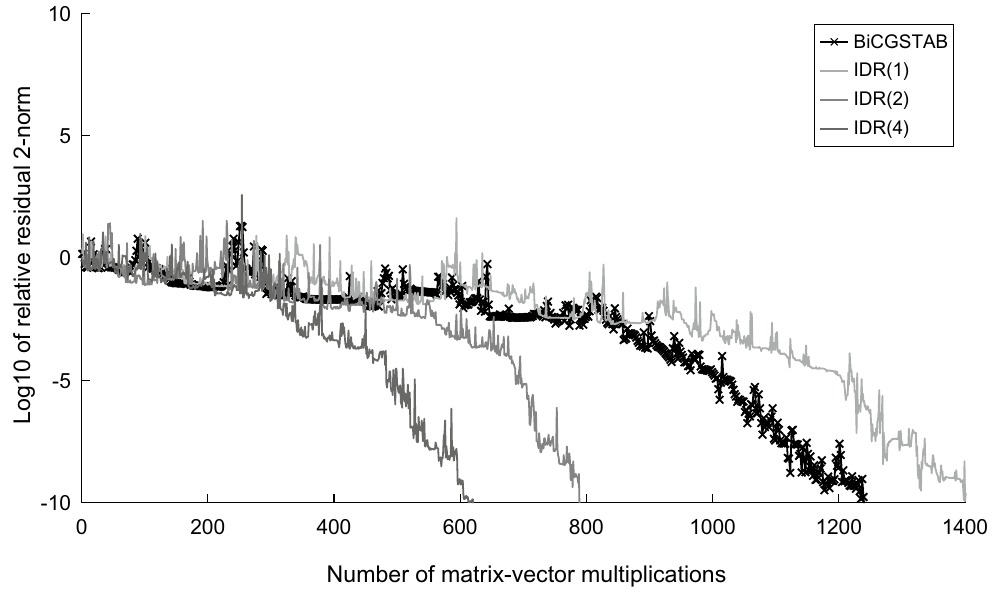
\includegraphics[width=.87\linewidth]{figures/idr-comparison.png}
\caption{{BiCGSTAB, IDR(1), IDR(2) 和 IDR(4) 的收敛历程}}\label{fig:idr-comparison}\end{figure}
% block: block-idr-heading page:152 type:subsection
\subsubsection{{块诱导降维 (块 IDR($s$)) 方法}}\label{subsec:block-idr-method}
{块 IDR($s$) 方法 \BookCite{46} 是 IDR($s$) 方法的推广, 用以求解形如下式的块线性方程组}
\begin{equation}\label{eq:block-linear-system}AX=B,\end{equation}
{其中 $A\in\mathbb C^{N\times N}$, $B\in\mathbb C^{N\times m}$, 且 $m$ 通常远小于 $N$.}
{在介绍块 IDR($s$) 方法的理论之前, 先在下列定义之后简要描述块 Krylov 子空间方法的框架:}
% block: block-krylov-definition page:152 type:definition
\par\Needspace{3\baselineskip}
\begin{Definition}{{块 Krylov 子空间}}\label{def:block-krylov-subspace}
{设 $V\in\mathbb C^{N\times m}$. 则由下式定义的 $\mathcal K_n(A,V)\subset\mathbb C^{N\times m}$}
\[\begin{aligned}\mathcal K_n(A,V)&:=\{VC_0+AVC_1+\cdots+A^{n-1}VC_{n-1}:C_0,C_1,\ldots,C_{n-1}\in\mathbb C^{m\times m}\}\\&(=\operatorname{block\ span}\{V,AV,\ldots,A^{n-1}V\})\end{aligned}\]
{称为关于 $A$ 和 $V$ 的块 Krylov 子空间.}
\end{Definition}
% block: block-krylov-sum-definition page:152 type:definition
\par\Needspace{3\baselineskip}
\begin{Definition}{{Krylov 子空间之和}}\label{def:block-krylov-sum}
{设 $V=[\bm v_1,\bm v_2,\ldots,\bm v_m]\in\mathbb C^{N\times m}$. 则 $\mathcal B_n(A,V)\subset\mathbb C^N$ 定义为}
\[\begin{aligned}\mathcal B_n(A,V)&:=\mathcal K_n(A,\bm v_1)+\mathcal K_n(A,\bm v_2)+\cdots+\mathcal K_n(A,\bm v_m)\\&=\{V\bm c_0+AV\bm c_1+\cdots+A^{n-1}V\bm c_{n-1}:\bm c_0,\bm c_1,\ldots,\bm c_{n-1}\in\mathbb C^m\}.\end{aligned}\]
\end{Definition}
% block: block-krylov-grade-definition page:152 type:definition
\par\Needspace{3\baselineskip}
\begin{Definition}{{块 Krylov 子空间的阶}}\label{def:block-krylov-grade}
{满足下式的最小数 $n$}
\[\dim(\mathcal B_n(A,V))=\dim(\mathcal B_{n+1}(A,V))\]
{称为 $A$ 关于 $V$ 的块阶, 记为 $\nu(V,A)$.}
\end{Definition}
% block: block-grade-reduction-remark page:152 type:remark
\par\Needspace{3\baselineskip}
\begin{Remark}\label{rem:block-grade-scalar-reduction}
{Definition\ \ref{def:block-krylov-subspace} 和 Definition\ \ref{def:block-krylov-grade} 是 Definition\ \ref{def:krylov-subspace} 和 Definition\ \ref{def:krylov-grade} 的推广. 事实上, 若 $m=1$, 这些定义就与 Definition\ \ref{def:krylov-subspace} 和 Definition\ \ref{def:krylov-grade} 相同.}
\end{Remark}
% block: block-krylov-framework pages:152,153 type:ordinary-paragraph
{现在描述块 Krylov 子空间方法的框架. 设 $X_0\in\mathbb C^{N\times s}$ 为初始猜测, $R_0:=B-AX_0$ 为相应的初始残差矩阵. 则块 Krylov 子空间方法按下式寻找第 $n$ 个近似解 $X_n$:}
\[X_n=X_0+Z_n,\quad Z_n\in\mathcal K_n(A,R_0).\]
{相应的残差矩阵为}
\[R_n=B-AX_n=R_0-AZ_n\in\mathcal K_{n+1}(A,R_0).\]
{确定 $Z_n$ 就得到各种块 Krylov 子空间方法, 例如,}
\begin{itemize}
\item{块 CG 方法:} $R_n\perp\mathcal B_n(A,R_0)$.
\item{块 COCG 方法:} $R_n\perp\overline{\mathcal B_n(A,R_0)}$.
\item{块 BiCG 方法:} $R_n\perp\mathcal B_n(A^{\mathrm H},R_0^{*})$.
\end{itemize}
{这里 $R_0^{*}$ 为初始影子残差矩阵,}\footnote{{实际中通常取 $R_0^{*}=R_0$, 或将 $R_0^{*}$ 设为随机矩阵.}}
{符号 $R_n\perp\mathcal B_n(A,V)$ 表示 $R_n$ 的所有列向量都与 $\mathcal B_n(A,V)$ 正交.}
% block: block-krylov-history page:153 type:ordinary-paragraph
{\leavevmode\phantomsection\label{idx:chapter-03-section-03:block-krylov-history}这里简要回顾块 Krylov 子空间方法的历史. 1980 年, O’Leary 在 \BookCite{142} 中提出块 BiCG 方法 (及块 CG 方法). 1990 年, Vital 在 \BookCite{202} 中提出块 GMRES 方法. 1997 年提出了基于 QMR 方法的块 Krylov 子空间方法 \BookCite{65}, \BookCite{157}. 2003 年, Guennouni 等提出块 BiCGSTAB 方法 \BookCite{86}. 2011 年, Du 等提出块 IDR($s$) 方法 \BookCite{46}. 其他块 Krylov 子空间方法见 \BookCite{153}, \BookCite{181}, \BookCite{182}, \BookCite{210}.}
{现在转向块 IDR($s$) 方法的推导. 块 IDR($s$) 方法基于下述定理 (见 \BookCite{46}), 它是 Theorem\ \ref{thm:idr-dimension-reduction} 的轻微修改.}
% block: block-idr-theorem page:153 type:theorem
\par\Needspace{14\baselineskip}
\begin{Theorem}\label{thm:block-idr-dimension-reduction}
{设 $A$ 为 $\mathbb C^{N\times N}$ 中的任意矩阵, $\bm v_0$ 为 $\mathbb C^N$ 中的任意非零向量, 并设 $\mathcal G_0=\mathcal B_{\nu(R_0,A)}(A,R_0)$. 设 $\mathcal S$ 表示 $\mathbb C^N$ 的任意 (真) 子空间, 使 $\mathcal S$ 和 $\mathcal G_0$ 不具有共同的非平凡不变子空间,}\footnote{{这意味着 $\mathcal S\cap\mathcal G_0$ 不包含 $A$ 的任何特征向量, 平凡不变子空间为 $\{\bm0\}$.}}
{并定义序列 $\mathcal G_j$, $j=1,2,\ldots$ 为}
\begin{equation}\label{eq:block-idr-subspace-recurrence}\mathcal G_j=(I-\omega_jA)(\mathcal G_{j-1}\cap\mathcal S),\end{equation}
{其中 $\omega_j$ 为非零标量. 则:}
\begin{enumerate}[label=(\arabic*)]
\item $\mathcal G_j\subset\mathcal G_{j-1}$ {对所有 $j>0$ 成立.}
\item $\mathcal G_j=\{\bm0\}$ {对某个 $j\le N$ 成立.}
\end{enumerate}\end{Theorem}
% block: block-idr-theorem-proof pages:153,154 type:proof
\begin{Proof}
{Theorem\ \ref{thm:idr-dimension-reduction} 和 Theorem\ \ref{thm:block-idr-dimension-reduction} 的唯一区别在于 $\mathcal G_0$ 的定义, 即 $\mathcal G_0=\mathcal K_N(A,\bm v_0)$ 或 $\mathcal G_0=\mathcal B_{\nu(R_0,A)}(A,R_0)$. 在 Theorem\ \ref{thm:idr-dimension-reduction}-(1) 的证明中, $\mathcal G_0=\mathcal K_N(A,\bm v_0)$ 仅用于证明 $\mathcal G_1\subset\mathcal G_0$. 因此只需证明 $\mathcal G_1\subset\mathcal G_0$. 由 $\mathcal G_0=\mathcal B_{\nu(R_0,A)}(A,R_0)$ 有 $(I-\omega_1A)\mathcal G_0\subset\mathcal G_0$, 因为对于给定的 $\bm v\in(I-\omega_1A)\mathcal G_0=(I-\omega_1A)\mathcal B_{\nu(R_0,A)}(A,R_0)$, 有}
\[\begin{aligned}\bm v&=(I-\omega_1A)(R_0\bm c_0+AR_0\bm c_1+\cdots+A^{\nu(R_0,A)-1}R_0\bm c_{\nu(R_0,A)-1})\\&=(I-\omega_1A)R_0\bm c_0+(I-\omega_1A)AR_0\bm c_1+\cdots+(I-\omega_1A)A^{\nu(R_0,A)-1}R_0\bm c_{\nu(R_0,A)-1}\\&=R_0\bm d_0+AR_0\bm d_1+\cdots+A^{\nu(R_0,A)-1}R_0\bm d_{\nu(R_0,A)-1}+A^{\nu(R_0,A)}R_0\bm d_{\nu(R_0,A)}\\&=R_0\widetilde{\bm d}_0+AR_0\widetilde{\bm d}_1+\cdots+A^{\nu(R_0,A)-1}R_0\widetilde{\bm d}_{\nu(R_0,A)-1}\\&\in\mathcal G_0.\end{aligned}\]
{因此 $\mathcal G_1=(I-\omega_1A)(\mathcal G_0\cap\mathcal S)\subset(I-\omega_1A)\mathcal G_0\subset\mathcal G_0$.}
{按照 Theorem\ \ref{thm:idr-dimension-reduction}-(2) 的证明并使用 $\dim\mathcal G_0\le N$, 即可证明 Theorem\ \ref{thm:block-idr-dimension-reduction}-(2).}
\par\nopagebreak[4]
\end{Proof}
% block: block-idr-dimension-corollary page:154 type:corollary
{与 Corollary\ \ref{cor:idr-dimension-step} 类似, 有下列事实:}
\par\Needspace{3\baselineskip}
\begin{Corollary}\label{cor:block-idr-dimension-step}
{对于给定的 $s,m\ge1$, 设 $\mathcal S$ 为 $\mathbb C^N$ 的子空间, 且 $\dim(\mathcal S)=N-sm$. 若 $\mathcal G_{i-1}+\mathcal S=\mathbb C^N$ 且 $(I-\omega_jA)$ 非奇异, 则}
\[\dim(\mathcal G_j)=\dim(\mathcal G_{j-1})-sm.\]
\end{Corollary}
{Corollary\ \ref{cor:idr-dimension-step} 与 Corollary\ \ref{cor:block-idr-dimension-step} 的区别在于参数 $m$. 参数 $m$ 对应于 $AX=B$ 的右端项个数, 其中 $B$ 为 $N$ 行 $m$ 列的矩阵.}
% block: block-idr-subspace-choice page:154 type:ordinary-paragraph
{下面解释块 IDR($s$) 方法. 块 IDR($s$) 方法对 $k=0,1,\ldots$ 生成残差矩阵 $R_k=B-AX_k$, 使得:}
\begin{enumerate}
\item{对 $j=0,1,2,\ldots$, $R_{j(s+1)},R_{j(s+1)+1},\ldots,R_{j(s+1)+s}$ 的所有列向量属于 \eqref{eq:block-idr-subspace-recurrence} 中的 $\mathcal G_j$;}
\item{选择 \eqref{eq:block-idr-subspace-recurrence} 中的子空间 $\mathcal S$, 使 $\dim\mathcal S=N-sm$.}
\end{enumerate}
{设 $S=[\bm s_1,\bm s_2,\ldots,\bm s_{sm}]\in\mathbb C^{N\times sm}$. 则子空间 $\mathcal S$ 的标准选择如下:}
\[\mathcal S=\operatorname{span}\{S\}^{\perp}=\operatorname{span}\{\bm s_1,\bm s_2,\ldots,\bm s_{sm}\}^{\perp},\]
{其中 $S\in\mathbb C^{N\times sm}$ 的所有列向量线性无关, 因此容易看出 $\dim\mathcal S=N-sm$.}
% block: block-idr-two-residuals page:154 type:ordinary-paragraph
{现在简要说明 $s=2$ 的块 IDR($s$) 方法. 对 $j=0,1,2$, 块 IDR(2) 方法产生下列残差矩阵:}
\[R_0,R_1,R_2,\quad R_3,R_4,R_5,\quad R_6,R_7,R_8,\]
{其中 $R_0,R_1,R_2$ 的所有列向量属于 $\mathcal G_0$, $R_3,R_4,R_5$ 的所有列向量属于 $\mathcal G_1$, $R_3,R_4,R_5$ 的所有列向量属于 $\mathcal G_2$.}
{下面在 $R_0,R_1,R_2$ 的所有列向量属于 $\mathcal G_0$ 的假设下, 说明如何从 $R_0,R_1,R_2$ 得到 $R_3,R_4,R_5$. 与 IDR($s$) 方法类似, 下列定义对块 IDR($s$) 方法有用:}
\begin{equation}\label{eq:block-idr-residual-differences}\Delta R_k:=R_{k+1}-R_k,\quad dR_k^{\blacksquare}:=[\Delta R_k,\Delta R_{k+1}],\quad C_k=(S^{\mathrm H}dR_k^{\blacksquare})^{-1}S^{\mathrm H}R_{k+2}.\end{equation}
{下列矩阵 $V_0$ 的所有列向量位于 $\mathcal G_0\cap\mathcal S$ 中:}
\[V_0=R_2-dR_0^{\blacksquare}C_0,\quad\operatorname{Im}(V_0)\subset\mathcal G_0\cap\mathcal S\]
% block: block-idr-first-reduced-residual page:155 type:ordinary-paragraph
{因为由 $R_0,R_1,R_2$ 的所有列向量属于 $\mathcal G_0$ 这一假设, $R_2\in\mathbb C^{N\times m}$ 和 $dR_0\in\mathbb C^{N\times2m}$ 的所有列向量属于 $\mathcal G_0$; 又由关系 $S^{\mathrm H}V_0=O$, $V_0$ 的所有列向量也属于 $\mathcal S$, 其中 $O$ 为 $2m\times m$ 零矩阵. 这里 $\operatorname{Im}(V_0)$ 为 $V_0$ 的像, 即 $V_0$ 的所有列向量张成的子空间.}
{由 \eqref{eq:block-idr-subspace-recurrence}, 列向量属于 $\mathcal G_1$ 的残差矩阵 $R_3$ 可按下式产生}
\begin{equation}\label{eq:block-idr-first-reduced-residual}R_3=(I-\omega_0A)V_0,\quad\operatorname{Im}(R_3)\subset\mathcal G_1,\end{equation}
{其中通常选择 $\omega_0$ 使 $\|R_3\|_{\mathrm F}$ 达到极小值,}\footnote{{对 $R=(r_{i,j})\in\mathbb C^{N\times m}$, 符号 $\|R\|_{\mathrm F}:=(\sum_{i=1}^N\sum_{j=1}^m\bar r_{i,j}r_{i,j})^{1/2}$ 称为 $R$ 的 Frobenius 范数; 对方阵 $A=(a_{i,j})\in\mathbb C^{N\times N}$, 符号 $\operatorname{Tr}(A):=\sum_{i=1}^Na_{i,i}$ 称为 $A$ 的迹.}}
{即,}
\[\omega_0=\frac{\operatorname{Tr}(T_0^{\mathrm H}V_0)}{\operatorname{Tr}(T_0^{\mathrm H}T_0)},\quad T_0:=AV_0.\]
% block: frobenius-minimization-proposition page:155 type:proposition
{Frobenius 范数的极小化来自下列事实:}
\par\Needspace{3\baselineskip}
\begin{Proposition}\label{prop:frobenius-scalar-minimization}
{设 $V,W\in\mathbb C^{m\times n}$. 则下列极小化问题:}
\[\min_{\omega\in\mathbb C}\|V-\omega W\|_{\mathrm F}\]
{可由下式求解}
\[\omega=\frac{\operatorname{Tr}(W^{\mathrm H}V)}{\operatorname{Tr}(W^{\mathrm H}W)}.\]
\end{Proposition}
% block: frobenius-minimization-proof page:155 type:proof
\begin{Proof}
{设 $V=[\bm v_1,\ldots,\bm v_n]$, $W=[\bm w_1,\ldots,\bm w_n]$, 则使用}
\[\bm v:=\operatorname{vec}(V)=\begin{bmatrix}\bm v_1\\\vdots\\\bm v_n\end{bmatrix},\quad\bm w:=\operatorname{vec}(W)=\begin{bmatrix}\bm w_1\\\vdots\\\bm w_n\end{bmatrix}\]
{得到 $\|V-\omega W\|_{\mathrm F}=\|\bm v-\omega\bm w\|$. 因而由 \eqref{eq:scalar-residual-minimizer}, 极小化参数为}
\[\omega=\frac{\bm w^{\mathrm H}\bm v}{\bm w^{\mathrm H}\bm w}=\frac{\operatorname{Tr}(W^{\mathrm H}V)}{\operatorname{Tr}(W^{\mathrm H}W)},\]
{证明完毕.}
\par\nopagebreak[4]
\end{Proof}
% block: block-idr-next-residuals pages:155,156 type:ordinary-paragraph
{与 IDR($s$) 方法中 $\bm r_3$ 和 $\bm r_4$ 的推导类似, 按下式得到 $R_3$ 和 $R_4$:}
\[\begin{aligned}V_1&=R_3-dR_1^{\blacksquare}C_1,&\operatorname{Im}(V_1)&\subset\mathcal G_0\cap\mathcal S,\\R_4&=(I-\omega_0A)V_1,&\operatorname{Im}(R_4)&\subset\mathcal G_1,\\V_2&=R_4-dR_2^{\blacksquare}C_2,&\operatorname{Im}(V_2)&\subset\mathcal G_0\cap\mathcal S,\\R_5&=(I-\omega_0A)V_2,&\operatorname{Im}(R_5)&\subset\mathcal G_1.\end{aligned}\]
{由上述计算, 得到残差矩阵 $R_k$ ($k=0,\ldots,5$), 使得}
\[\begin{aligned}\operatorname{Im}(R_k)&\subset\mathcal G_0\quad\text{for }k=0,1,2,\\\operatorname{Im}(R_k)&\subset\mathcal G_1\quad\text{for }k=3,4,5.\end{aligned}\]
% block: block-idr-solution-extraction page:156 type:ordinary-paragraph
{接着说明如何从 $X_0,X_1,X_2$ 得到近似解矩阵 $X_3,X_4,X_5$. 令}
\[\Delta X_k:=X_{k+1}-X_k,\qquad dX_k^{\blacksquare}:=[\Delta X_k,\Delta X_{k+1}].\]
{则按下式得到 $X_3$:}
\[\begin{aligned}R_3&=(I-\omega_0A)V_0=R_2-dR_0^{\blacksquare}C_0-\omega_0AV_0\\&\Leftrightarrow B-AX_3=B-AX_2-dR_0^{\blacksquare}C_0-\omega_0AV_0\\&\Leftrightarrow X_3=X_2+A^{-1}dR_0^{\blacksquare}C_0+\omega_0V_0\\&\Leftrightarrow X_3=X_2-dX_0^{\blacksquare}C_0+\omega_0V_0.\end{aligned}\]
{类似地,}
\[\begin{aligned}X_4&=X_3-dX_1^{\blacksquare}C_1+\omega_0V_1,\\X_5&=X_4-dX_2^{\blacksquare}C_2+\omega_0V_2.\end{aligned}\]
{已说明在 $s=2$ 的块 IDR($s$) 方法中, 如何从 $k=0,1,2$ 的 $R_k$ 和 $X_k$ 得到 $k=3,4,5$ 的 $R_k$ 和 $X_k$. 按照上述推导, 得到 Algorithm\ \ref{alg:block-idr} 中的块 IDR($s$) 方法. 此外, 块 IDR($s$) 方法的预条件版本见 Algorithm\ \ref{alg:preconditioned-block-idr}. 注意, 符号 ``$B(:,\ell)$'' 表示矩阵 $B$ 的第 $\ell$ 列, 符号 ``$\Delta X(:,im+1:(i+1)m)$'' 表示矩阵 $\Delta X$ 的第 $(im+1)$, $(im+2)$, $\ldots$, $(i+1)m$ 列.}
% block: block-idr-cost-remark pages:156,157 type:remark
\par\Needspace{3\baselineskip}
\begin{Remark}\label{rem:block-idr-matvec-bound}
{由 Corollary\ \ref{cor:block-idr-dimension-step}, 维数的减少量通常为 $sm$, 即 $\dim(\mathcal G_j)=\dim(\mathcal G_{j-1})-sm$, 块 IDR($s$) 方法需要 $m(s+1)$ 次矩阵向量乘法. 因此, 在精确运算中, 块 IDR($s$) 方法得到精确解矩阵所需的矩阵向量乘法总次数至多为 $m(s+1)\times N/sm=N+N/s$, 不依赖于块大小 $m$. 注意, 若对 $AX=B$ 应用 IDR($s$) 方法 (即 $A\bm x_1=\bm b_1,A\bm x_2=\bm b_2,\ldots,A\bm x_m=\bm b_m$), 则 IDR($s$) 方法所需的矩阵向量乘法次数至多为 $m(N+N/s)$, 是块 IDR($s$) 方法的 $m$ 倍.}
\end{Remark}
% block: block-idr-bicgstab-remark page:157 type:remark
{由下面的注, 块 IDR($s$) 方法可视为块 BiCGSTAB 方法的推广.}
\par\Needspace{3\baselineskip}
\begin{Remark}\label{rem:block-idr-bicgstab-equivalence}
{块 IDR(1) 方法和块 BiCGSTAB 方法在偶数步给出相同的残差向量.}
\end{Remark}
% block: block-idr-algorithm page:157 type:ordinary-paragraph
\begin{algorithm}[H]\caption{{块 IDR($s$) 方法}}\label{alg:block-idr}\begin{algorithmic}[1]
\Statex\textbf{Input:} $X_0\in\mathbb C^{N\times s},\ R_0=B-AX_0,\ P\in\mathbb C^{n\times sm}$
\Statex\textbf{Output:} $X_i$
\For{$i=0$ {至} $s-1$}
\State $V=AR_i,\quad\omega=\frac{\operatorname{Tr}(V^{\mathrm H}R_i)}{\operatorname{Tr}(V^{\mathrm H}V)}$
\State $\Delta X(:,im+1:(i+1)m)=\omega R_i,\quad\Delta R(:,im+1:(i+1)m)=-\omega V$
\State $X_{i+1}=X_i+\Delta X(:,im+1:(i+1)m),\quad R_{i+1}=R_i+\Delta R(:,im+1:(i+1)m)$
\EndFor
\State $j=1,\quad i=s$
\State $M=P^{\mathrm H}\Delta R,\quad H=P^{\mathrm H}R_i$
\While{$\max_{\ell\in\{1,2,\ldots,m\}}\frac{\|R_i(:,\ell)\|_{\mathrm F}}{\|B(:,\ell)\|_{\mathrm F}}>\epsilon$}
\For{$k=0$ {至} $s$}
\State{由 $MC=H$ 解出 $C$}
\State $Q=-\Delta RC,$
\State $V=R_i+Q$
\If{$k=0$}
\State $T=AV,\quad\omega=\frac{\operatorname{Tr}(T^{\mathrm H}V)}{\operatorname{Tr}(T^{\mathrm H}T)}$
\State $\Delta R(:,(j-1)m+1:jm)=Q-\omega T$
\State $\Delta X(:,(j-1)m+1:jm)=-\Delta XC+\omega V$
\Else
\State $\Delta X(:,(j-1)m+1:jm)=-\Delta XC+\omega V$
\State $\Delta R(:,(j-1)m+1:jm)=-A\Delta X(:,(j-1)m+1:jm)$
\EndIf
\State $R_{i+1}=R_i+\Delta R(:,(j-1)m+1:jm)$
\State $X_{i+1}=X_i+\Delta X(:,(j-1)m+1:jm)$
\State $\Delta M=P^{\mathrm H}\Delta R(:,(j-1)m+1:jm)$
\State $M(:,(j-1)m+1:jm)=\Delta M$
\State $H=H+\Delta M$
\State $i=i+1,\quad j=j+1$
\State $j=(j-1)\%s+1$ ({$\%$: 取模运算, 即 $a\%n=r$, 其中 $a=mn+r$.})
\EndFor\EndWhile\end{algorithmic}\end{algorithm}
% block: preconditioned-block-idr-algorithm page:158 type:ordinary-paragraph
\begin{algorithm}[H]\caption{{预条件块 IDR($s$) 方法}}\label{alg:preconditioned-block-idr}\begin{algorithmic}[1]
\Statex\textbf{Input:} $X_0\in\mathbb C^{N\times s},\ R_0=B-AX_0,\ P\in\mathbb C^{n\times sm}$
\Statex\textbf{Input:} $X_0=KX_0$ ($K$: {预条件矩阵})
\Statex\textbf{Output:} $X_i$
\For{$i=0$ {至} $s-1$}
\State $W=K^{-1}R_i$
\State $V=AW,\quad\omega=\frac{\operatorname{Tr}((K_1^{-1}V)^{\mathrm H}K_1^{-1}R_i)}{\operatorname{Tr}((K_1^{-1}V)^{\mathrm H}K_1^{-1}V)}$
\State $\Delta X(:,im+1:(i+1)m)=\omega R_i,\quad\Delta R(:,im+1:(i+1)m)=-\omega V$
\State $X_{i+1}=X_i+\Delta X(:,im+1:(i+1)m),\quad R_{i+1}=R_i+\Delta R(:,im+1:(i+1)m)$
\EndFor
\State $j=1,\quad i=s$
\State $M=P^{\mathrm H}\Delta R,\quad H=P^{\mathrm H}R_i$
\While{$\max_{\ell\in\{1,2,\ldots,m\}}\frac{\|R_i(:,\ell)\|_{\mathrm F}}{\|B(:,\ell)\|_{\mathrm F}}>\epsilon$}
\For{$k=0$ {至} $s$}
\State{由 $MC=H$ 解出 $C$}
\State $Q=-\Delta RC$
\State $V=R_i+Q$
\If{$k=0$}
\State $T=AK^{-1}V,\quad\omega=\frac{\operatorname{Tr}((K_1^{-1}T)^{\mathrm H}K_1^{-1}V)}{\operatorname{Tr}((K_1^{-1}T)^{\mathrm H}K_1^{-1}T)}$
\State $\Delta R(:,(j-1)m+1:jm)=Q-\omega T$
\State $\Delta X(:,(j-1)m+1:jm)=-\Delta XC+\omega V$
\Else
\State $\Delta X(:,(j-1)m+1:jm)=-\Delta XC+\omega V$
\State $\Delta R(:,(j-1)m+1:jm)=-AK^{-1}\Delta X(:,(j-1)m+1:jm)$
\EndIf
\State $R_{i+1}=R_i+\Delta R(:,(j-1)m+1:jm)$
\State $X_{i+1}=X_i+\Delta X(:,(j-1)m+1:jm)$
\State $\Delta M=P^{\mathrm H}\Delta R(:,(j-1)m+1:jm)$
\State $M(:,(j-1)m+1:jm)=\Delta M$
\State $H=H+\Delta M$
\State $i=i+1,\quad j=j+1$
\State $j=(j-1)\%s+1$ ({$\%$: 取模运算, 即 $a\%n=r$, 其中 $a=mn+r$.})
\EndFor\EndWhile
\State $X_i=K^{-1}X_i$
\end{algorithmic}\end{algorithm}
